% Бүлэг 2
\chapter{Улаанбаатар хотын дугуйн замын crowd-sourcing веб системийн шинжилгээ} % Бүлгийн нэр
\label{Chapter2} % Энэ бүлэг рүү ишлэл хийх бол \ref{Chapter2} командыг ашигла

\section{Системийн үйл ажиллагааны тухай дэлгэрэнгүй}
Энэхүү систем нь Улаанбаатар хотын дугуйн замын мэдээллийг олон нийтийн оролцоонд тулгуурлан цуглуулж, газрын зураг дээр визуалчилж харуулдаг crowd-sourcing веб юм. Хэрэглэгчид замын хэсгүүдэд нөхцлийн тэмдэглэгээ хийх, аюулын болон сонирхолтой цэгүүдийг (POI) газрын зурагт байрлуулах, бусад хэрэглэгчдийн оруулсан мэдээллийг харах боломжтой \cite{Reference3}. Систем нь олон хэрэглэгчийн оруулсан саналуудыг нэгтгэж тухайн замын сегментийн давамгай нөхцлийг автоматаар тодорхойлдог crowd aggregation механизмтай. Үүний үр дүнд замын аюулгүй байдлыг ногоон (bike lane байгаа), шар (боломжтой), улаан (боломжгүй) гэсэн гурван ангиллаар үнэлж газрын зурагт өнгөөр харуулна. Мөн хэрэглэгч эхлэл болон төгсгөлийн цэгийг сонгосон тохиолдолд тус өгөгдөлд тулгуурлан аюулгүй маршрутыг автоматаар тооцоолж санал болгоно. Хэрэглэгчид имейл, нууц үгээр бүртгэл үүсгэн системд нэвтэрвэл өөрийн оруулсан POI -ууд, явсан замын тэмдэглэгээнүүд хадгалагдаж, профайлаас удирдах боломжтой. Системийн POI төрлүүд нь дараах 6 ангилалд хуваагдана. \say{Аюултай бүс (Danger), Дугуйн зам байхгүй хэсэг (No Bike Lane), Замын эвдрэл (Road Damage), Машины буруу зогсолт (Parking Problem), Дугуй засварлах цэг (Bike Repair), Дугуй зогсоох цэг (Bike Parking).} Замын дэд бүтцийн нөхцлийг 1-р зэрэглэлийн тусгаарлагдсан дугуйн замаас 6-р зэрэглэлийн дундаа ашиглах зам хүртэл 6 түвшингээр ангилж бүртгэнэ.

\section{Системийг ашиглах хэрэглэгчид}
\paragraph{} Тус системийг нас, хүйс хамаарахгүйгээр Улаанбаатар хотод дугуй унадаг, дугуйн зам хайдаг, эсвэл дугуйн замын мэдээлэл оруулахыг хүссэн интернэтэд холбогдсон хэн бүр ашиглаж болно. Системийг ашиглаж буй хэрэглэгчдийг бүртгэлгүй хэрэглэгч (зочин), бүртгэлтэй хэрэглэгч болон админ гэж 3 ангилна.

\section{Функцийн шаардлага}
Бүртгэлгүй хэрэглэгчийн (зочин) функцийн шаардлага
\begin{enumerate}
    \item Зочин газрын зураг дээрх замын нөхцлийг (ногоон/шар/улаан) харж болно.
    \item Зочин газрын зураг дээрх POI -уудыг харж, дэлгэрэнгүй мэдээллийг үзэж болно.
    \item Зочин эхлэл, төгсгөлийн цэг сонгож аюулгүй маршрут гаргуулж болно.
\end{enumerate}
Бүртгэлтэй хэрэглэгчийн функцийн шаардлага
\begin{enumerate}
    \item Хэрэглэгч системд имейл хаяг, нууц үг гэсэн талбаруудыг бөглөж бүртгүүлнэ.
    \item Бүртгэгдсэн имейлээр системд нэвтэрнэ.
    \item Газрын зураг дээр замын сегмент сонгож ногоон/шар/улаан өнгийн нөхцлийг тэмдэглэж болно.
    \item Газрын зураг дээр POI байрлуулж, төрөл (Danger / No Bike Lane / Road Damage / Parking Problem / Bike Repair / Bike Parking) сонгох болон тайлбар, зураг хавсаргах боломжтой.
    \item POI дээр upvote/downvote санал өгч болно (нэг POI -д нэг санал).
    \item GPS бичлэгийг 'Start Route' товчоор эхлүүлж, 'Stop Route' товчоор зогсоох боломжтой.
    \item Явсан замаа GPX файл хэлбэрээр экспортлож татаж авах боломжтой.
    \item Хэрэглэгч өөрийн профайлаас нийт явсан км, route тоо, POI тоог харах боломжтой.
    \item Хэрэглэгч өөрийн оруулсан POI -г засах эсвэл устгаж болно.
\end{enumerate}
Админы функцийн шаардлага
\begin{enumerate}
    \item Админ хүлээгдэж буй (pending) POI -уудыг батлах эсвэл татгалзах боломжтой.
    \item Админ системийн ерөнхий статистикийг dashboard -аас харж болно (нийт route, POI тоо, асуудалтай газар, bike lane coverage).
    \item Админ хэрэглэгчдийн жагсаалтыг харж, ban/unban үйлдэл хийх боломжтой.
    \item Админ замын сегмент болон POI өгөгдлийг CSV/Excel хэлбэрээр экспортлож болно.
\end{enumerate}
Системийн функцийн шаардлага
\begin{enumerate}
    \item Систем олон хэрэглэгчийн оруулсан саналыг нэгтгэж сегмент бүрийн давамгай нөхцлийг автоматаар тооцоолно (crowd aggregation).
    \item Систем хэрэглэгчийн сонгосон эхлэл, төгсгөлийн цэгт суурилан OSRM серверээр маршрут тооцоолж, аюулгүй болон хурдан гэсэн хоёр төрлийн маршрутыг харуулна.
    \item Ижил байршилд 3 ба түүнээс дээш POI цугларвал тухайн бүсийг тодруулж харуулна.
    \item Бүртгэл үүсгэсэн хэрэглэгчид JWT токен олгож stateless authentication хийнэ.
    \item Хэрэглэгчийн роль (зочин/хэрэглэгч/админ) -ийн дагуу зөвшөөрөгдсөн үйлдлүүдийг хязгаарлана (RBAC).
\end{enumerate}

\section{Функцийн бус шаардлага}
\begin{enumerate}
    \item Хэрэглэгчийн интерфейс ойлгомжтой, Bootstrap 5 -д суурилсан responsive загвартай байна.
    \item Бүртгэлтэй хэрэглэгчийн нууц үг хамгийн багадаа 6 ширхэг том, жижиг үсэг, тоо, тэмдэгтийг агуулсан байна.
    \item POI -д хавсаргах зураг 5MB хүртэлх хэмжээтэй, JPG, JPEG, PNG өргөтгөлтэй байна.
    \item Front-end болон back-end хооронд солилцох API хүсэлтийн хариу нь Application JSON форматтай байна.
    \item GPS байршлын мэдээлэл 1 секунд тутамд шинэчлэгдэнэ. Газрын зураг 2 секундын дотор ачаалагдана. Маршрут тооцоолол 3 секундын дотор гүйцэтгэгдэнэ.
    \item Системийн uptime 99\% -иас доош байж болохгүй, өдөр бүр өгөгдлийн санг автоматаар backup хийнэ.
    \item Хэрэглэгчийн мэдээлэл JWT auth, bcrypt нууц үг hash, RBAC, CSRF, XSS хамгаалалт ашиглан хадгалагдана.
    \item Аюулын POI тойролтын радиус 50м -ээс хэтрэхгүй, маршрут зам сүлжээнд нийцэж тооцоологдоно.
    \item Package ба Import statements - Пакеж доторх классуудтай холбоотой нэр үгээр пакежийг нэрлэнэ.
    \item Class Header ба Declaration - Классын нэрийг тухайн класс дотор хийгдэж байгаа үйл ажиллагаатай холбоотой нэр үгээр нэрлэнэ.
    \item Method Headers ба Declarations - Метод буюу дэд функцийг тухайн функцийн гүйцэтгэх үйл үгээр нэрлэнэ.
    \item Функцийн дээд мөрөнд функцийн тайлбарыг коммент хэлбэрээр бичсэн байна.
    \item Хөгжүүлэлтийн туршид хөгжүүлэлтийн нэг phase бүр дээр нэгжийн тестийг хийдэг байна (test coverage 40\% -иас дээш).
\end{enumerate}

\section{Юзкейс диаграмм}
\paragraph{} Зураг \ref{fig:usecase} -д дүрслэгдсэн дугуйн замын crowd-sourcing веб системийн юзкейс диаграмм нь зочин, бүртгэлтэй хэрэглэгч, админ гэсэн 3 тоглогчид болон тэдгээрийн ашиглаж болох нийт юзкейсүүдийг агуулсан.
\begin{figure}[H]
    \centering
    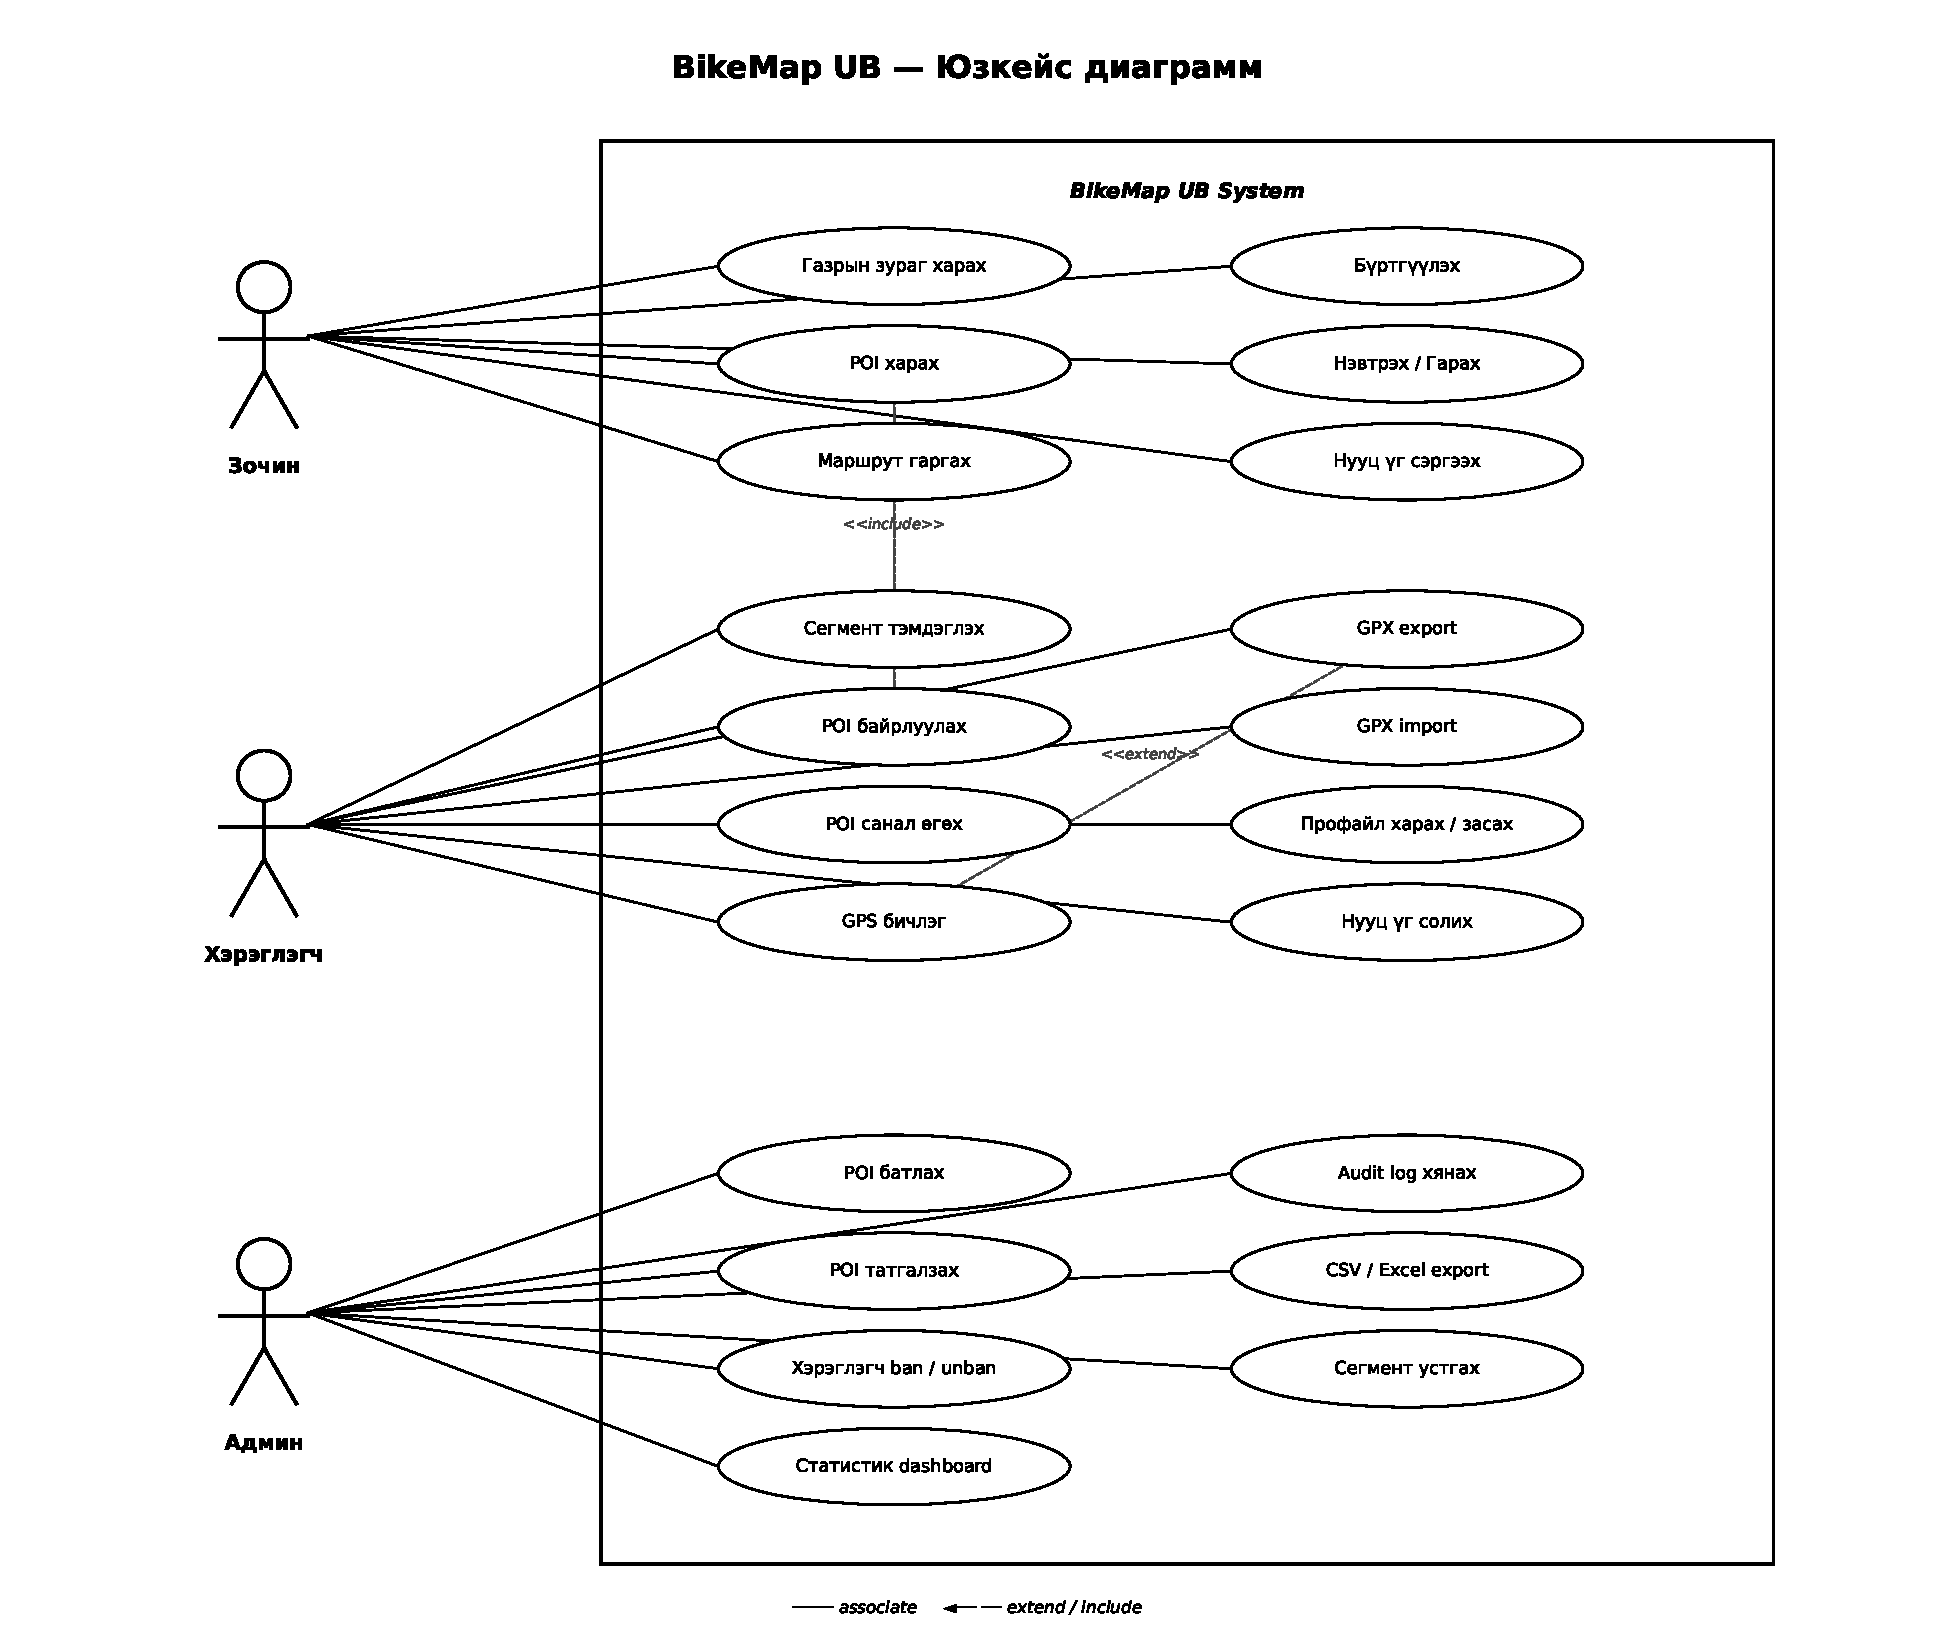
\includegraphics[scale=0.75]{Figures/chapter2/usecase.pdf}
    \caption{Юзкейс диаграмм}
    \label{fig:usecase}
\end{figure}

\section{Юзкейсийн тодорхойлолт}
\begin{longtable}{|r|p{11.5cm}|}
    \caption{Замын нөхцөл тэмдэглэх юзкейсийн тодорхойлолт}
	\label{table:usecase1}\\ \hline
	{Юзкейс:} & {Замын нөхцөл тэмдэглэх }\\ \hline
	{ID:} & {1 }\\ \hline
	{Үүсгэсэн:} & {Э.Батсайхан}\\ \hline
	{Үүсгэсэн огноо:} & {2026.02.10}\\ \hline
	{Үндсэн тоглогч:} & {Бүртгэлтэй хэрэглэгч}\\ \hline
	{Нэмэлт тоглогч:} & {Байхгүй}\\ \hline
	{Товч тайлбар:} & {Хэрэглэгч газрын зураг дээр замын сегмент сонгож тухайн хэсгийн нөхцлийг ногоон/шар/улаан өнгөөр тэмдэглэнэ.}\\ \hline
	{Өмнөх нөхцөл:} & {\begin{enumerate}[nosep]
	    \item Хэрэглэгч системд бүртгэлтэй болон нэвтэрсэн байна.
	    \item Газрын зураг ачаалагдсан байна.
	\end{enumerate}}\\ \hline
	{Үндсэн урсгал:} & {
	\begin{enumerate}[nosep]
	    \item Хэрэглэгч "Сегмент тэмдэглэх" товчийг дарна.
	    \item Газрын зураг дээр сегментийн эхлэл болон төгсгөлийн цэгийг сонгоно.
        \item Өнгөний сонголт UI харагдана (ногоон/шар/улаан).
        \item Хэрэглэгч нэг өнгийг сонгож, "Хадгалах" товчийг дарна.
	    \item if Тэмдэглэгээ амжилттай хадгалагдсан бол
	        \begin{enumerate}[nosep,label*=\arabic*.]
	            \item Газрын зурагт сегмент сонгосон өнгөөр зурагдана.
                \item Crowd aggregation алгоритм автоматаар ажиллана.
	        \end{enumerate}
	    \item if Тэмдэглэгээ амжилтгүй болсон бол
                \begin{enumerate}[nosep,label*=\arabic*.]
	        \item "Амжилтгүй, дахин оролдоно уу + алдааны мессеж" гэсэн pop-up харагдана.
                \item Сегмент газрын зурагт нэмэгдэхгүй.
	    \end{enumerate}
	\end{enumerate}}\\ \hline
	{Дараах нөхцөл:} & {\begin{enumerate}
	    \item Сегмент DB -д хадгалагдсан байна.
        \item Газрын зурагт өнгөтэй харагдана.
	\end{enumerate}}\\ \hline
	{Альтернатив урсгал:} & {Байхгүй.}\\ \hline
\end{longtable}

\begin{longtable}{|r|p{11.5cm}|}
    \caption{POI байрлуулах юзкейсийн тодорхойлолт}
	\label{table:usecase2}\\ \hline
	{Юзкейс:} & {POI байрлуулах}\\ \hline
	{ID:} & {2}\\ \hline
	{Үүсгэсэн:} & {Э.Батсайхан}\\ \hline
	{Үүсгэсэн огноо:} & {2026.02.10}\\ \hline
	{Үндсэн тоглогч:} & {Бүртгэлтэй хэрэглэгч}\\ \hline
	{Нэмэлт тоглогч:} & {Админ}\\ \hline
	{Товч тайлбар:} & {Хэрэглэгч газрын зураг дээр аюулын болон сонирхолтой цэг (POI) байрлуулна.}\\ \hline
	{Өмнөх нөхцөл:} & {\begin{enumerate}[nosep]
	    \item Хэрэглэгч системд бүртгэлтэй болон нэвтэрсэн байна.
        \item Газрын зураг ачаалагдсан байна.
	\end{enumerate}}\\ \hline
	{Үндсэн урсгал:} & {
	\begin{enumerate}[nosep]
	    \item Хэрэглэгч газрын зураг дээр POI байрлуулах цэгийг дарна.
	    \item POI төрөл сонгох UI харагдана (Danger / No Bike Lane / Road Damage / Parking Problem / Bike Repair / Bike Parking).
	    \item Хэрэглэгч төрлөө сонгож тайлбар бичнэ (заавал биш) болон зураг хавсаргана (заавал биш).
        \item "Хадгалах" товчийг дарна.
	    \item if POI үүсэхэд амжилттай бол
	        \begin{enumerate}[nosep,label*=\arabic*.]
	            \item POI 'хүлээгдэж буй' (pending) статустай DB -д хадгалагдана.
                \item Газрын зурагт POI -г харагдуулна (батлагдсаны дараа нийтэд харагдана).
                \item Админд батлуулах хүлээлгэлд орно.
	        \end{enumerate}
	    \item if POI үүсэхэд амжилтгүй болсон бол
                \begin{enumerate}[nosep,label*=\arabic*.]
	        \item "Амжилтгүй, дахин оролдоно уу + алдааны мессеж" гэсэн pop-up харагдана.
                \item POI үүсэхгүй.
	    \end{enumerate}
	\end{enumerate}}\\ \hline
	{Дараах нөхцөл:} & {\begin{enumerate}
	    \item POI хүлээгдэж буй статустай DB -д хадгалагдсан байна.
	\end{enumerate}}\\ \hline
	{Альтернатив урсгал:} & {Байхгүй.}\\ \hline
\end{longtable}

\begin{longtable}{|r|p{11.5cm}|}
    \caption{Аюулгүй маршрут гаргах юзкейсийн тодорхойлолт}
	\label{table:usecase3}\\ \hline
	{Юзкейс:} & {Аюулгүй маршрут гаргах}\\ \hline
	{ID:} & {3}\\ \hline
	{Үүсгэсэн:} & {Э.Батсайхан}\\ \hline
	{Үүсгэсэн огноо:} & {2026.02.10}\\ \hline
	{Үндсэн тоглогч:} & {Зочин эсвэл бүртгэлтэй хэрэглэгч}\\ \hline
	{Нэмэлт тоглогч:} & {Байхгүй}\\ \hline
	{Товч тайлбар:} & {Хэрэглэгч эхлэл болон төгсгөлийн цэгийг сонгож, аюулын байдлыг тооцсон ухаалаг маршрутыг харна.}\\ \hline
	{Өмнөх нөхцөл:} & {\begin{enumerate}[nosep]
	    \item Газрын зураг ачаалагдсан байна.
        \item OSRM сервер ажиллагаатай байна.
	\end{enumerate}}\\ \hline
	{Үндсэн урсгал:} & {
	\begin{enumerate}[nosep]
	    \item Хэрэглэгч "Маршрут гаргах" товчийг дарна.
	    \item Хэрэглэгч газрын зураг дээр эхлэл цэг A -г сонгоно.
        \item Хэрэглэгч төгсгөл цэг B -г сонгоно.
	    \item Хэрэглэгч маршрутын төрлийг сонгоно (Аюулгүй / Хурдан).
	    \item if Маршрут амжилттай тооцоологдсон бол
	        \begin{enumerate}[nosep,label*=\arabic*.]
	            \item Маршрут газрын зурагт ногоон/шар/улаан өнгөөр харагдана.
                \item Аюулын POI -уудыг тойрсон зам санал болгоно.
                \item Маршрутын урт болон тооцоолсон хугацаа UI -д харагдана.
	        \end{enumerate}
	    \item if Маршрут гаргахад амжилтгүй болсон бол
                \begin{enumerate}[nosep,label*=\arabic*.]
	        \item "Маршрут олдсонгүй + алдааны мессеж" гэсэн pop-up харагдана.
	    \end{enumerate}
	\end{enumerate}}\\ \hline
	{Дараах нөхцөл:} & {\begin{enumerate}
	    \item Хэрэглэгч маршрутыг газрын зурагт харсан байна.
	\end{enumerate}}\\ \hline
	{Альтернатив урсгал:} & {Хэрэглэгч "Хадгалах" товчоор маршрутаа хадгалж URL -ээр хуваалцаж болно.}\\ \hline
\end{longtable}

\section{Шинжилгээний класс диаграмм}
\paragraph{} Зураг \ref{fig:sh-class} дээрх системийн шинжилгээний шатны класс диаграмм нь системд үндсэн үүрэг гүйцэтгэх "control" төрөлтэй байж болох 6 классыг тодорхойлж тэдгээрийн хоорондын холбоо хамаарлыг дүрсэлсэн. \say{Crowd Aggregation} класс нь олон хэрэглэгчийн оруулсан сегментийн саналуудыг хүлээн авч, нэгтгэн боловсруулж давамгай нөхцлийг тооцоолох үүрэгтэй класс. \say{Smart Route} класс нь эхлэл, төгсгөлийн цэгийг хүлээн авч OSRM серверт хүсэлт илгээн, crowd aggregation болон POI өгөгдөлд тулгуурлан аюулгүй маршрутыг тооцоолно. \say{Сегмент} класс нь замын хэсгийн нөхцлийн тэмдэглэгээг үүсгэж, шинэчилж, хадгалах үүрэгтэй. \say{POI} класс нь хэрэглэгчийн оруулсан аюулын болон сонирхолтой цэгүүдийг үүсгэж, vote -ыг бүртгэх, статусыг удирдах үүрэгтэй. \say{Хэрэглэгч} класс нь хэрэглэгчийн мэдээлэл, статистик, профайлыг зохион байгуулдаг класс. \say{Бүртгэл} класс нь имейл, нууц үгээр бүртгэл үүсгэх, JWT токен олгох, RBAC -аар роль шалгах үүрэгтэй класс юм.
\begin{figure}[H]
    \centering
    % 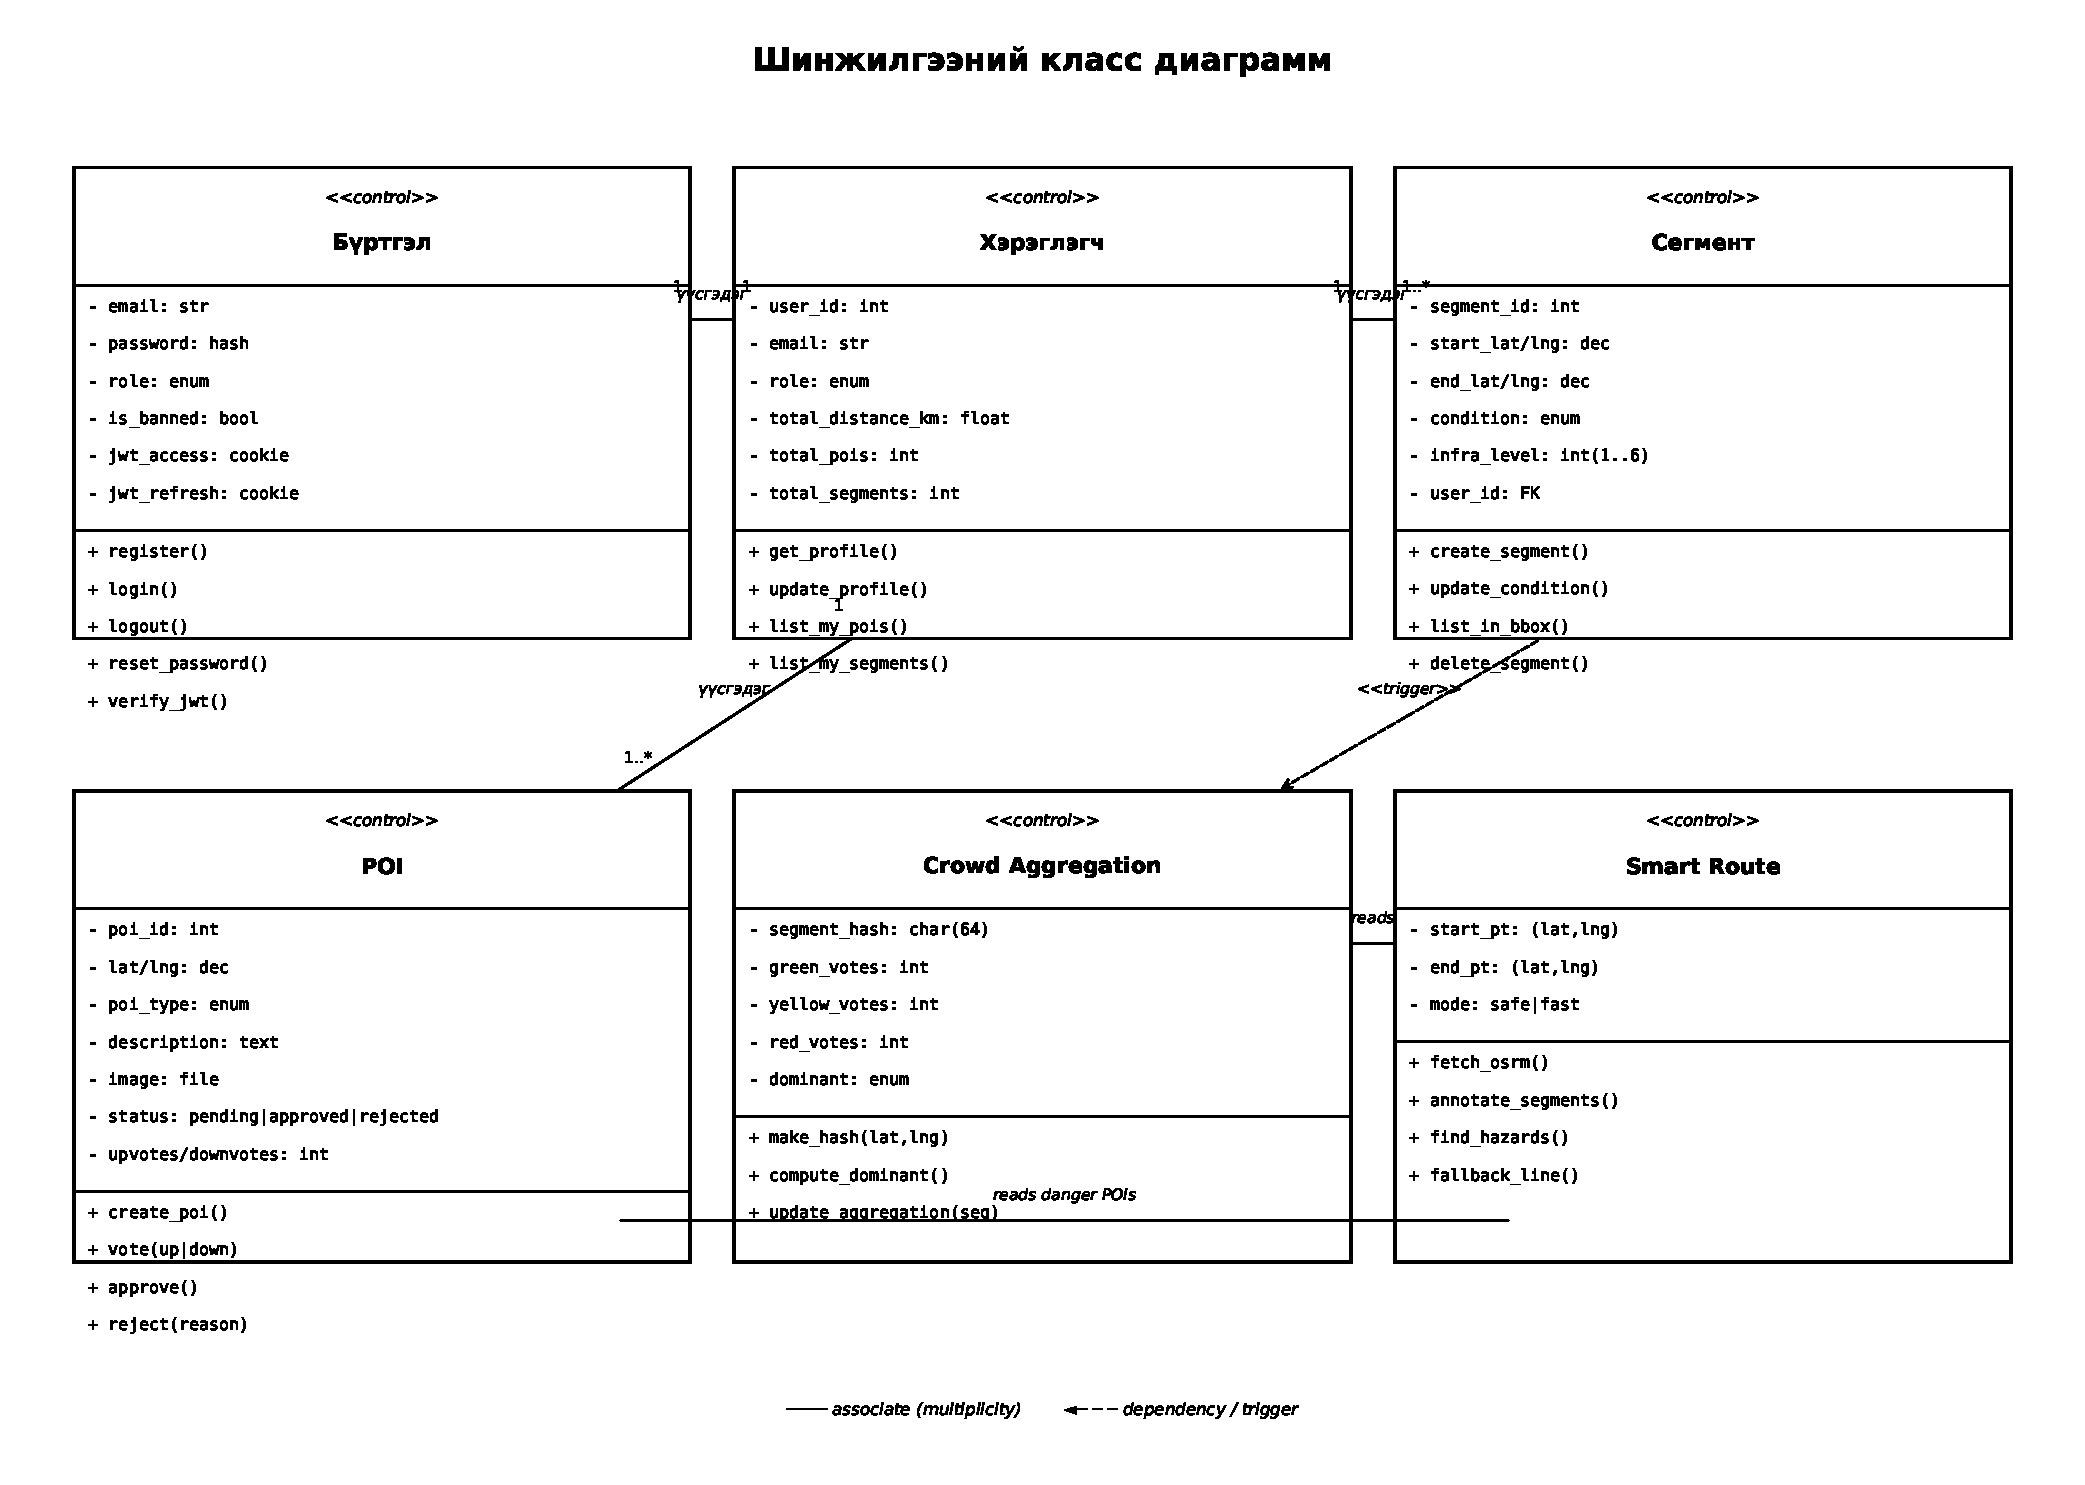
\includegraphics[scale=0.8]{Figures/chapter2/sh-class.pdf} % auto-commented: missing file
    \caption{Шинжилгээний класс диаграмм}
    \label{fig:sh-class}
\end{figure}

\section{Шинжилгээний дарааллын диаграмм}
\paragraph{}
Шинжилгээний класс диаграммд тодорхойлсон \say{control} төрлийн классуудын операторуудыг ашиглан \say{сегментийн нөхцөл тэмдэглэх}, \say{POI байрлуулах}, \say{маршрут гаргах}, \say{бүртгүүлэх}, \say{POI санал өгөх} гэсэн юзкейсүүдэд шинжилгээний шатны дарааллын диаграммыг гаргасан.
\par \noindent
Хэрэглэгч сегментийн нөхцөл тэмдэглэх үед дараах дарааллаар процесс явагдана. Хэрэглэгчийн хүсэлтийг \say{Сегмент} класс хүлээн авч, шинэ сегментийг үүсгэн \say{Crowd Aggregation} класс руу шинэчлэх дохио өгнө. Crowd Aggregation класс саналуудыг тоолж давамгай нөхцлийг тооцоолон үр дүнг буцаана. Зураг \ref{fig:segment-zh} -д дээрх дарааллыг агуулсан сегмент тэмдэглэх шинжилгээний дарааллын диаграммыг харуулж байна.
\begin{figure}[H]
    \centering
    % 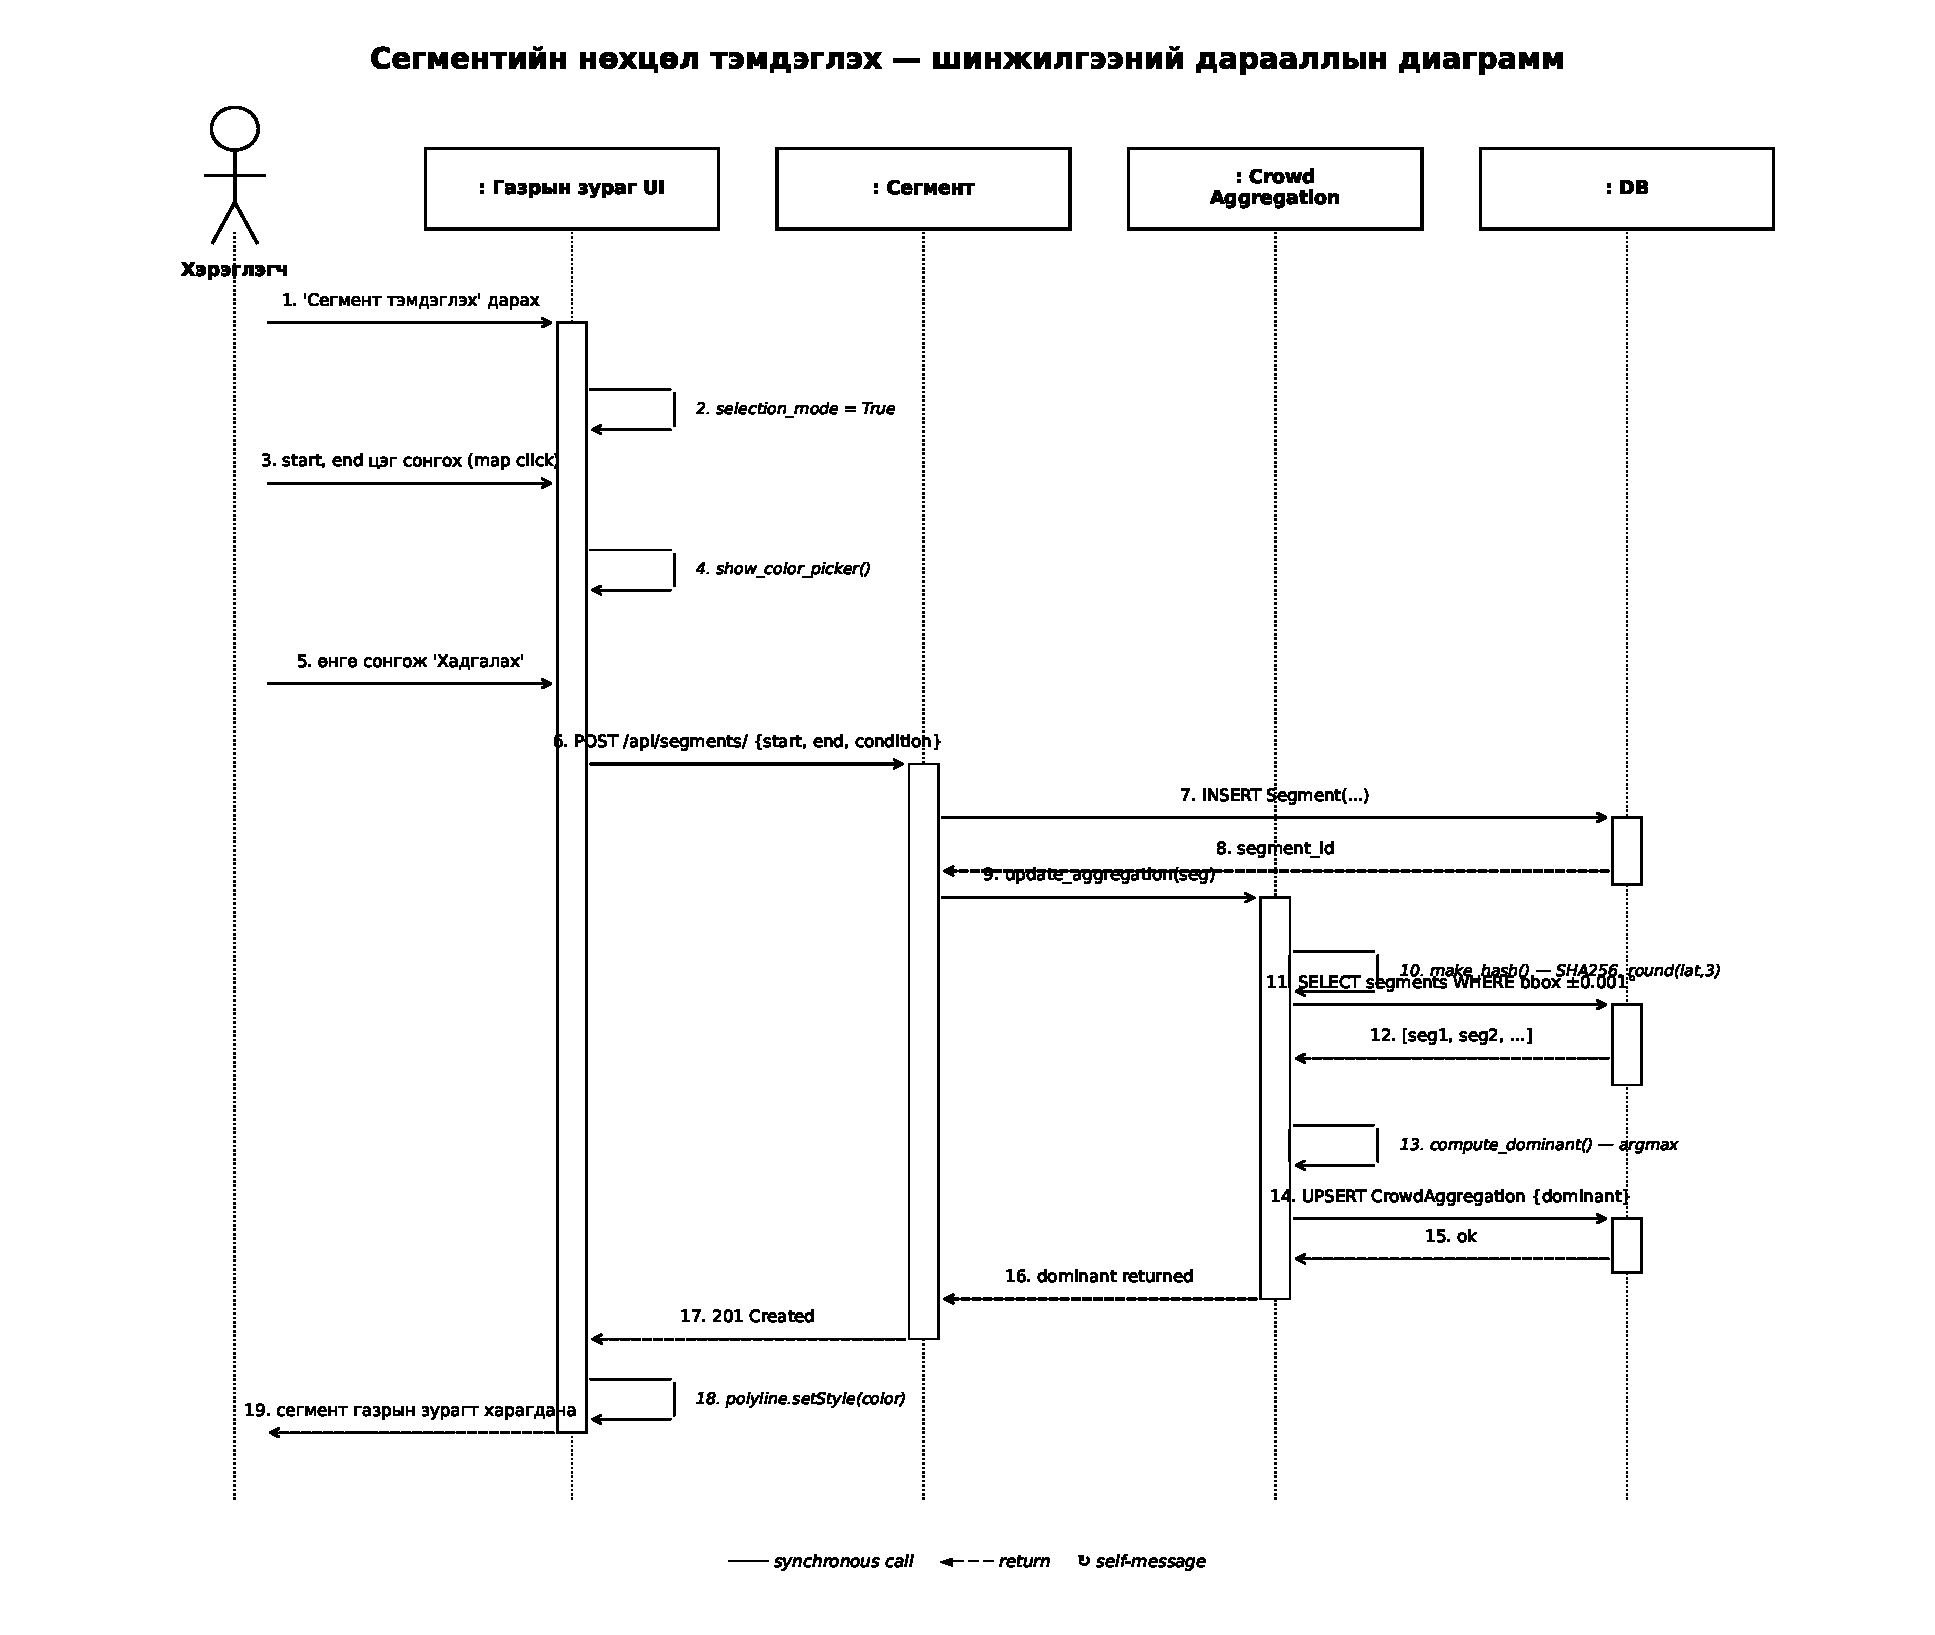
\includegraphics[scale=0.6]{Figures/chapter2/segment-zh.pdf} % auto-commented: missing file
    \caption{Сегментийн нөхцөл тэмдэглэх шинжилгээний дарааллын диаграмм}
    \label{fig:segment-zh}
\end{figure}
\par \noindent
Хэрэглэгч системд шинээр бүртгэл үүсгэх хүсэлтийг \say{Бүртгэл} класс хүлээн авч системд бүртгэлтэй эсэхийг шалгаад хэрэв бүртгэлгүй бол bcrypt -ээр нууц үг hash хийн \say{Хэрэглэгч} классаар дамжуулан шинэ хэрэглэгчийг системд бүртгэх хүсэлтийг явуулна. Амжилттай бол JWT токен үүсгэн буцаана. Дээрх процессыг Зураг \ref{fig:burtguuleh-zh} дээрх шинжилгээний дарааллын диаграммд дүрсэлсэн.
\begin{figure}[H]
    \centering
    % 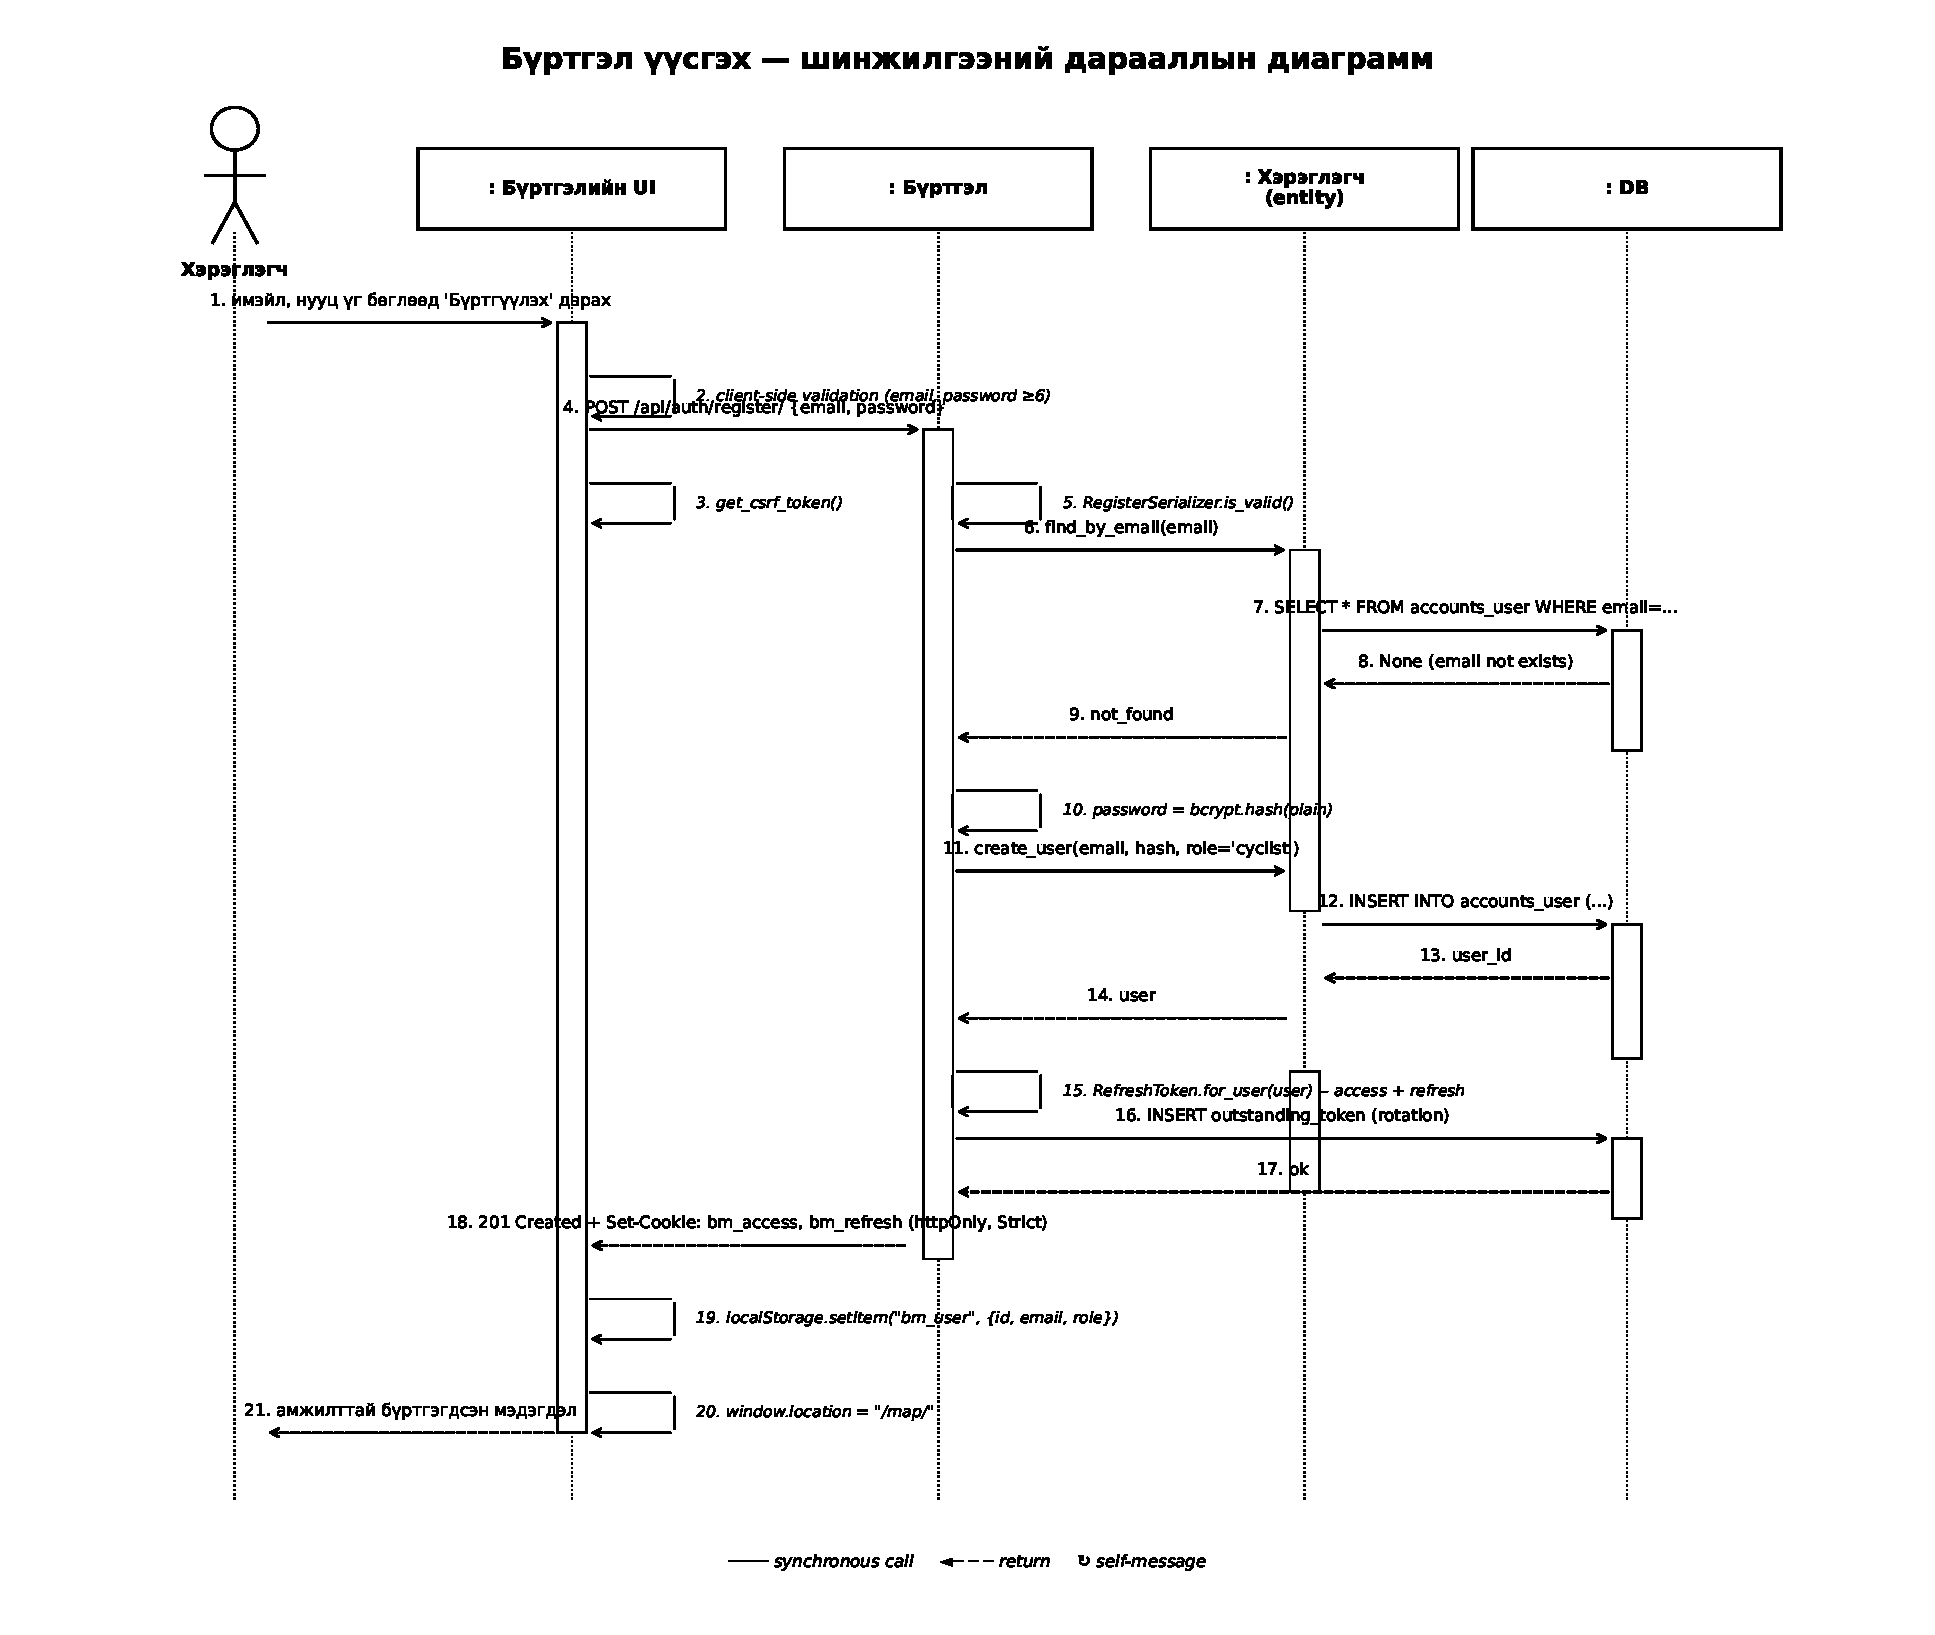
\includegraphics[scale=0.8]{Figures/chapter2/burtguuleh-zh.pdf} % auto-commented: missing file
    \caption{Бүртгэл үүсгэх шинжилгээний дарааллын диаграмм}
    \label{fig:burtguuleh-zh}
\end{figure}
\par \noindent
Хэрэглэгч A -аас B хүртэл маршрут гаргах үед \say{Smart Route} класс эхлэл, төгсгөлийн цэгийг хүлээн авч OSRM серверт хүсэлт илгээнэ. OSRM боломжит маршрутуудыг буцаасны дараа \say{Crowd Aggregation} класс руу хүсэлт илгээж сегмент бүрийн нөхцлийг авна. Үүний дараа \say{POI} классаас аюулын POI -уудыг авч нийт өртгийг тооцоолон хамгийн бага өртөгтэй маршрутыг буцаана. Дээрх процессыг Зураг \ref{fig:route-zh} дээрх шинжилгээний дарааллын диаграммд дүрсэлсэн.
\begin{figure}[H]
    \centering
    % 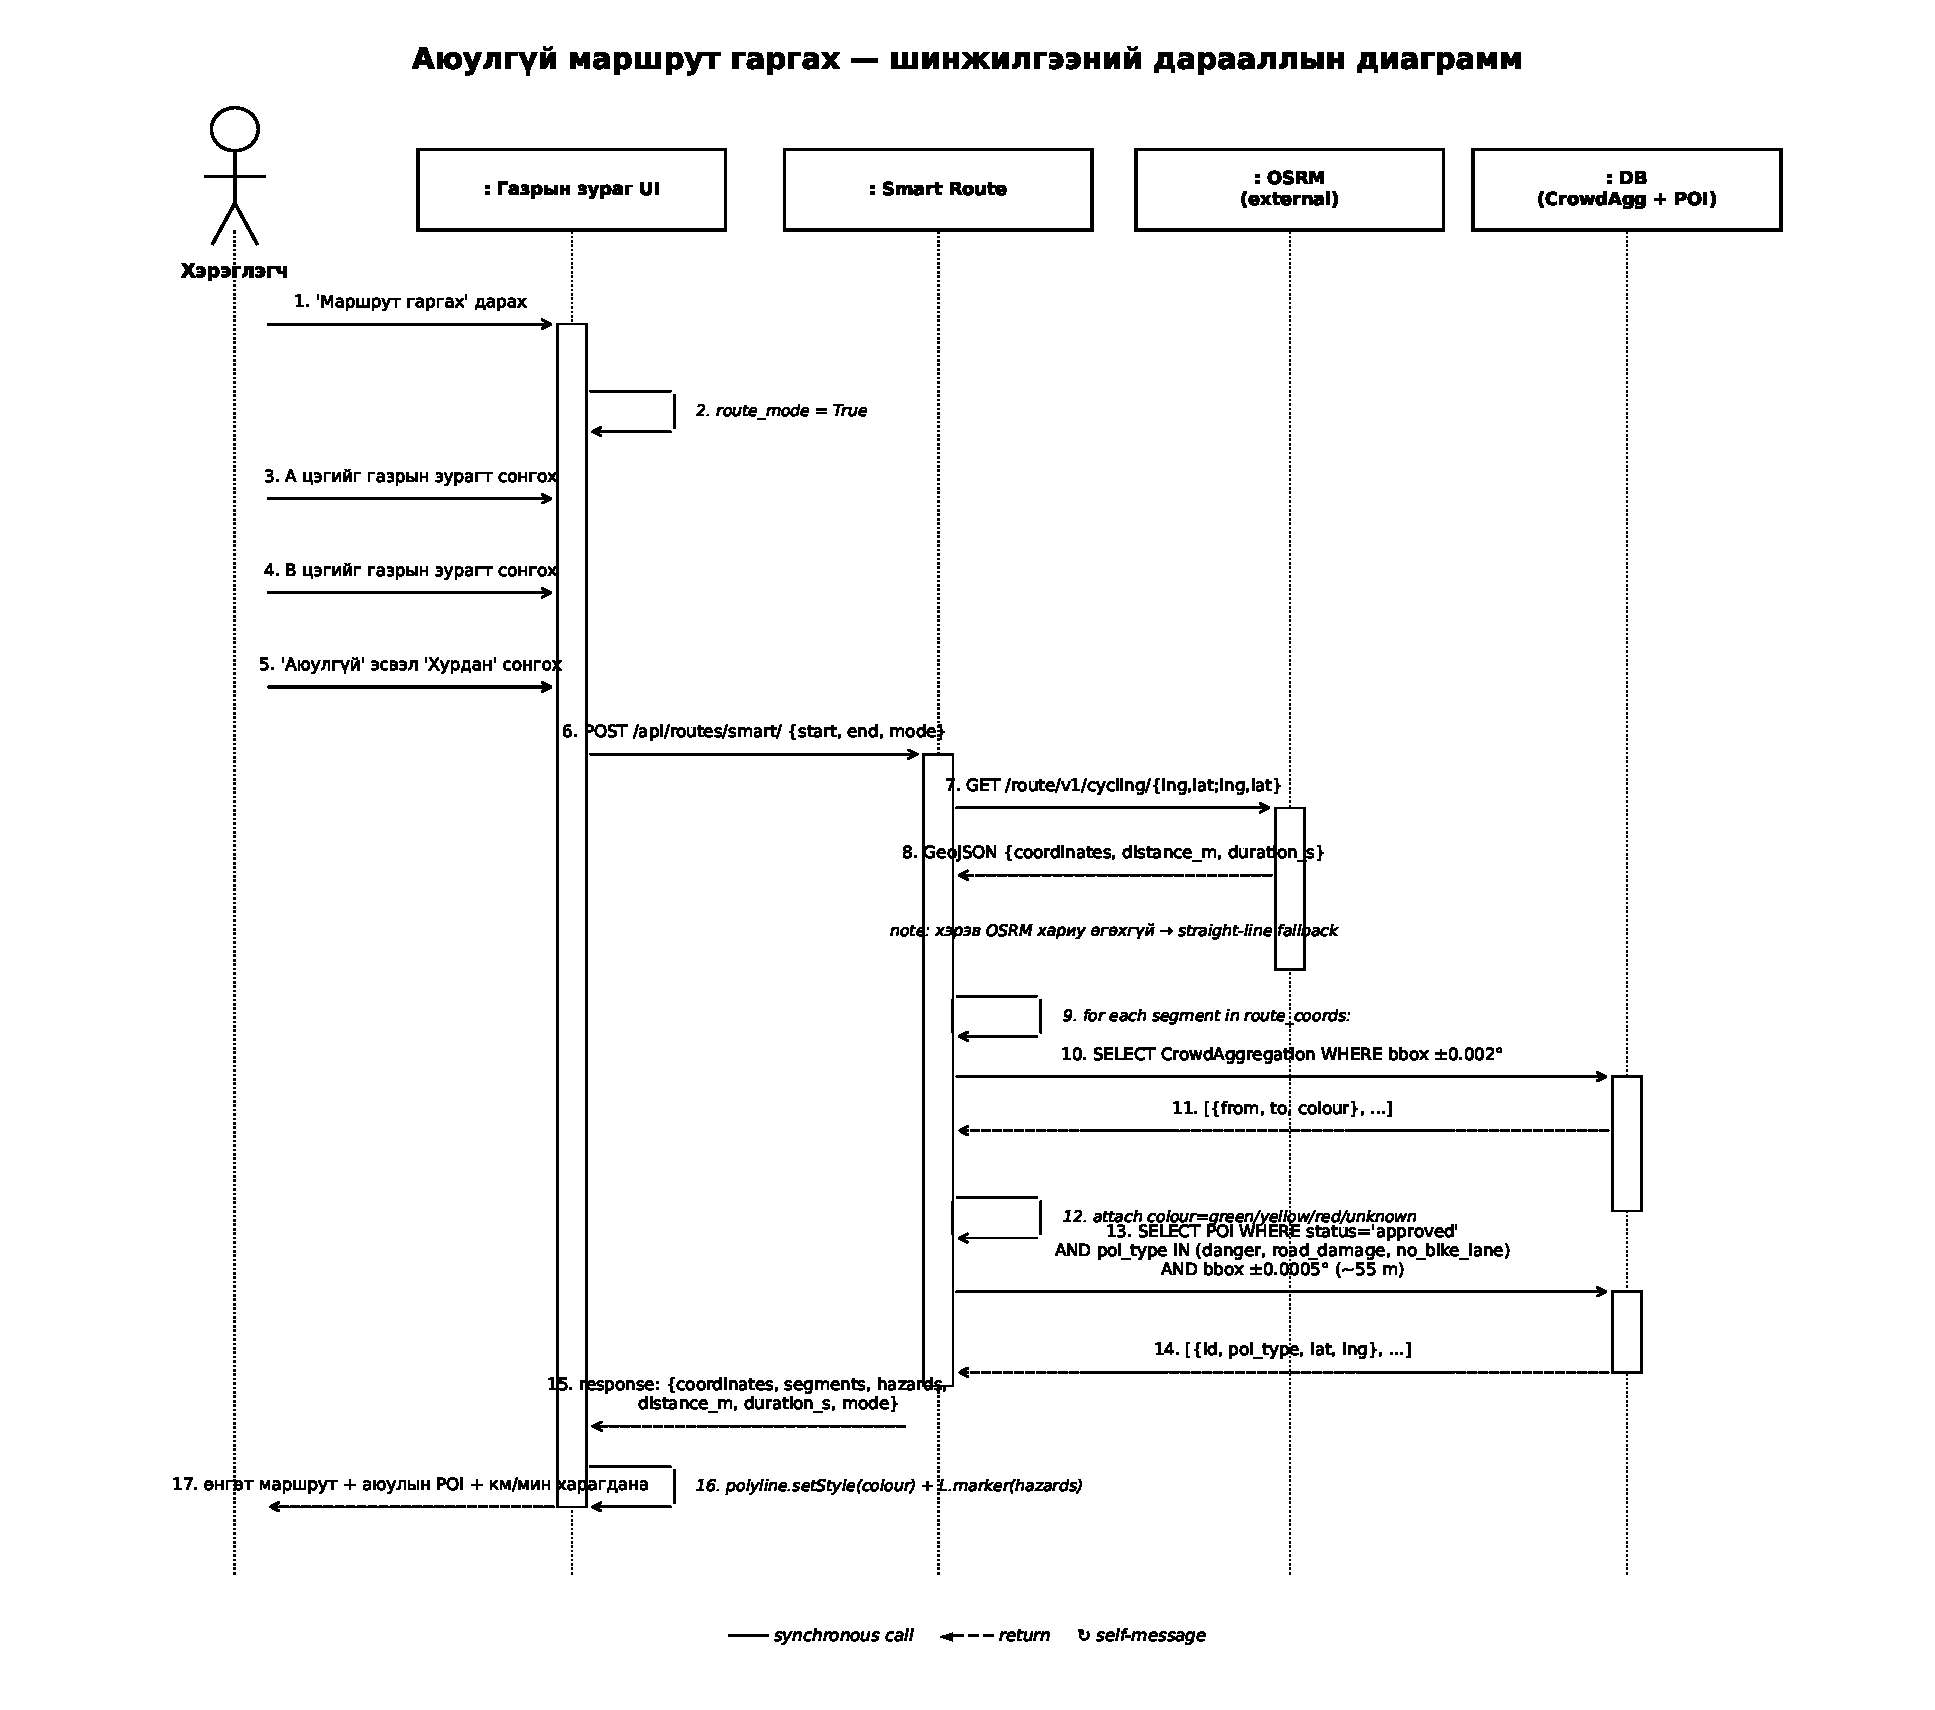
\includegraphics[scale=0.6]{Figures/chapter2/route-zh.pdf} % auto-commented: missing file
    \caption{Аюулгүй маршрут гаргах шинжилгээний дарааллын диаграмм}
    \label{fig:route-zh}
\end{figure}
\par \noindent

\section{Үйл ажиллагааны диаграмм}
\paragraph{}
Дугуйн замын crowd-sourcing веб системийн юзкейс диаграммд тодорхойлогдсон юзкейсүүдийн эхлэлээс төгсгөл хүртэлх үйлдлүүдийг дүрсэлсэн үйл ажиллагааны диаграммуудыг доор харуулав.
\par \noindent
Хэрэглэгч сегментийн нөхцөл тэмдэглэх үйл ажиллагаа нь хэрэглэгч системд нэвтэрснээр эхэлнэ. Хэрэглэгч "Сегмент тэмдэглэх" товчийг дарж газрын зураг дээр сегментийн эхлэл болон төгсгөл цэг сонгоно. Дараа нь нөхцлийн өнгийг (ногоон/шар/улаан) сонгож хадгална. Систем хадгалалт амжилттай эсэхийг шалгана; амжилттай бол газрын зурагт сонгосон өнгөөр харагдана, амжилтгүй бол хэрэглэгч дахин оролдох боломжтой. Дээрх процессыг Зураг \ref{fig:ua-segment} -н сегментийн нөхцөл тэмдэглэх үйл ажиллагааны диаграммаас харж болно.
\begin{figure}[H]
    \centering
    % 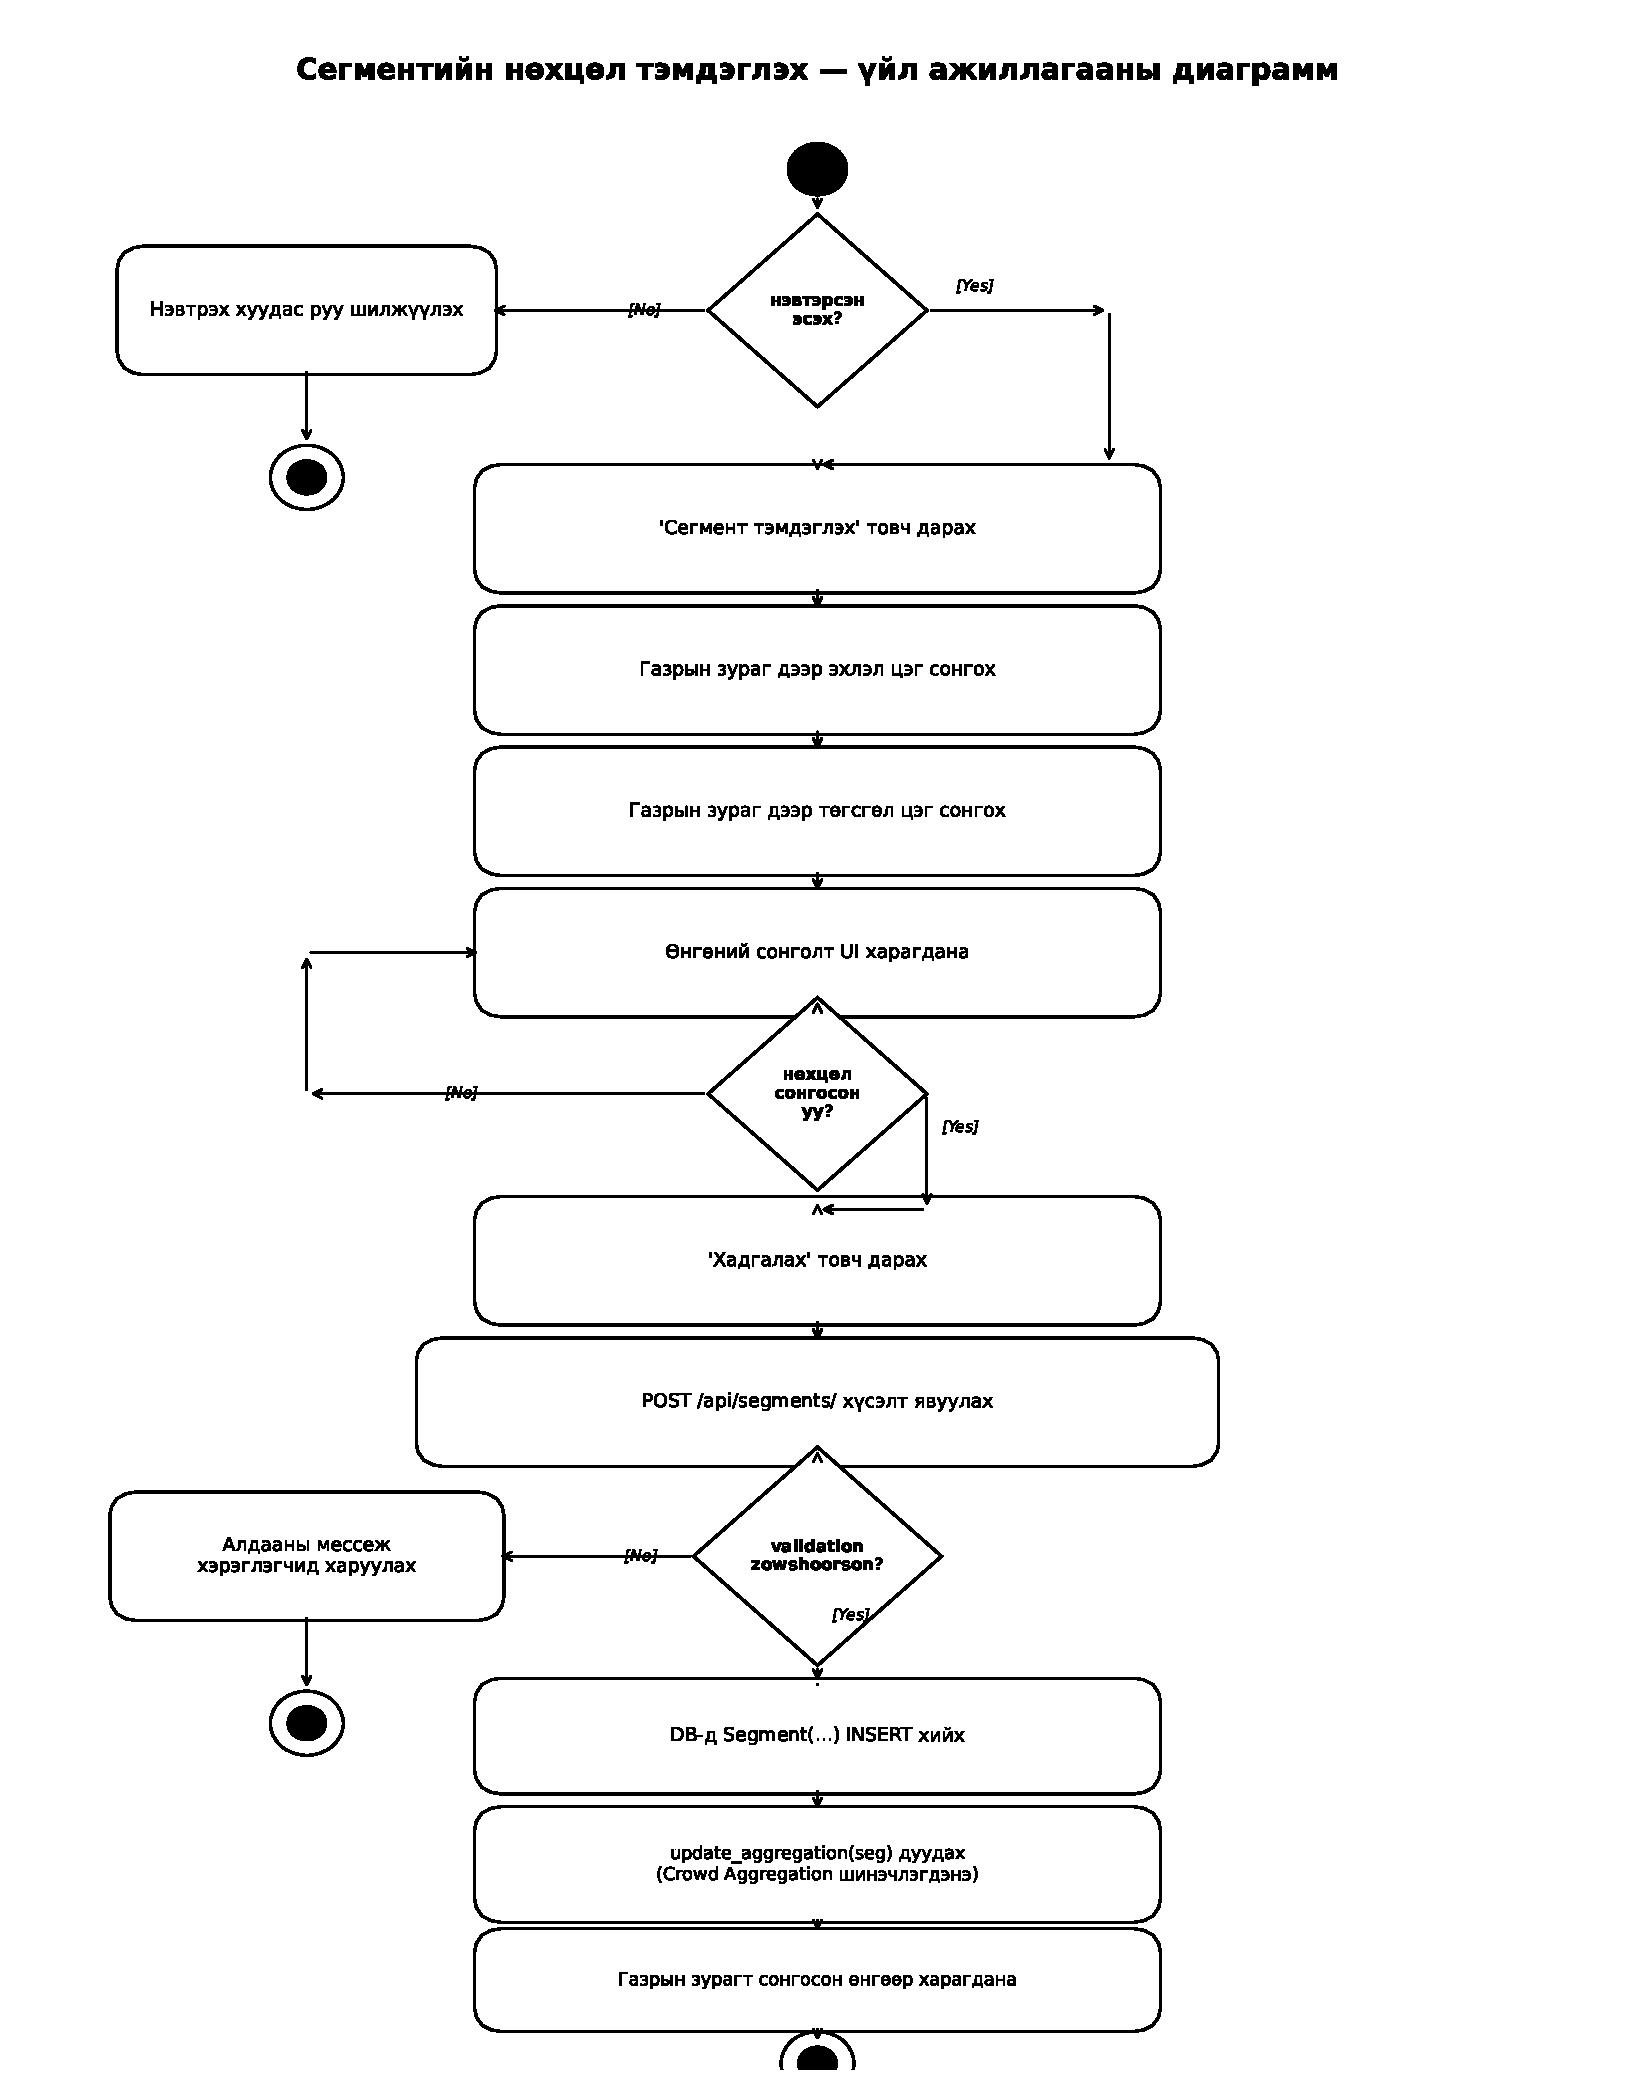
\includegraphics[scale=0.65]{Figures/chapter2/ua-segment.pdf} % auto-commented: missing file
    \caption{Сегментийн нөхцөл тэмдэглэх үйл ажиллагааны диаграмм}
    \label{fig:ua-segment}
\end{figure}
\par \noindent
POI байрлуулах үйл ажиллагаа нь хэрэглэгч газрын зураг дээр цэг сонгох үйлдлээс эхэлнэ. POI төрлийг сонгож тайлбар бичээд (заавал биш) зураг хавсаргана (заавал биш). Систем оролтыг шалган pending статустай DB -д хадгална. Админ батлах хүртэл нийтэд харагдахгүй. Дээрх процессыг Зураг \ref{fig:ua-poi} -н POI байрлуулах үйл ажиллагааны диаграммаас харж болно.
\begin{figure}[H]
    \centering
    % 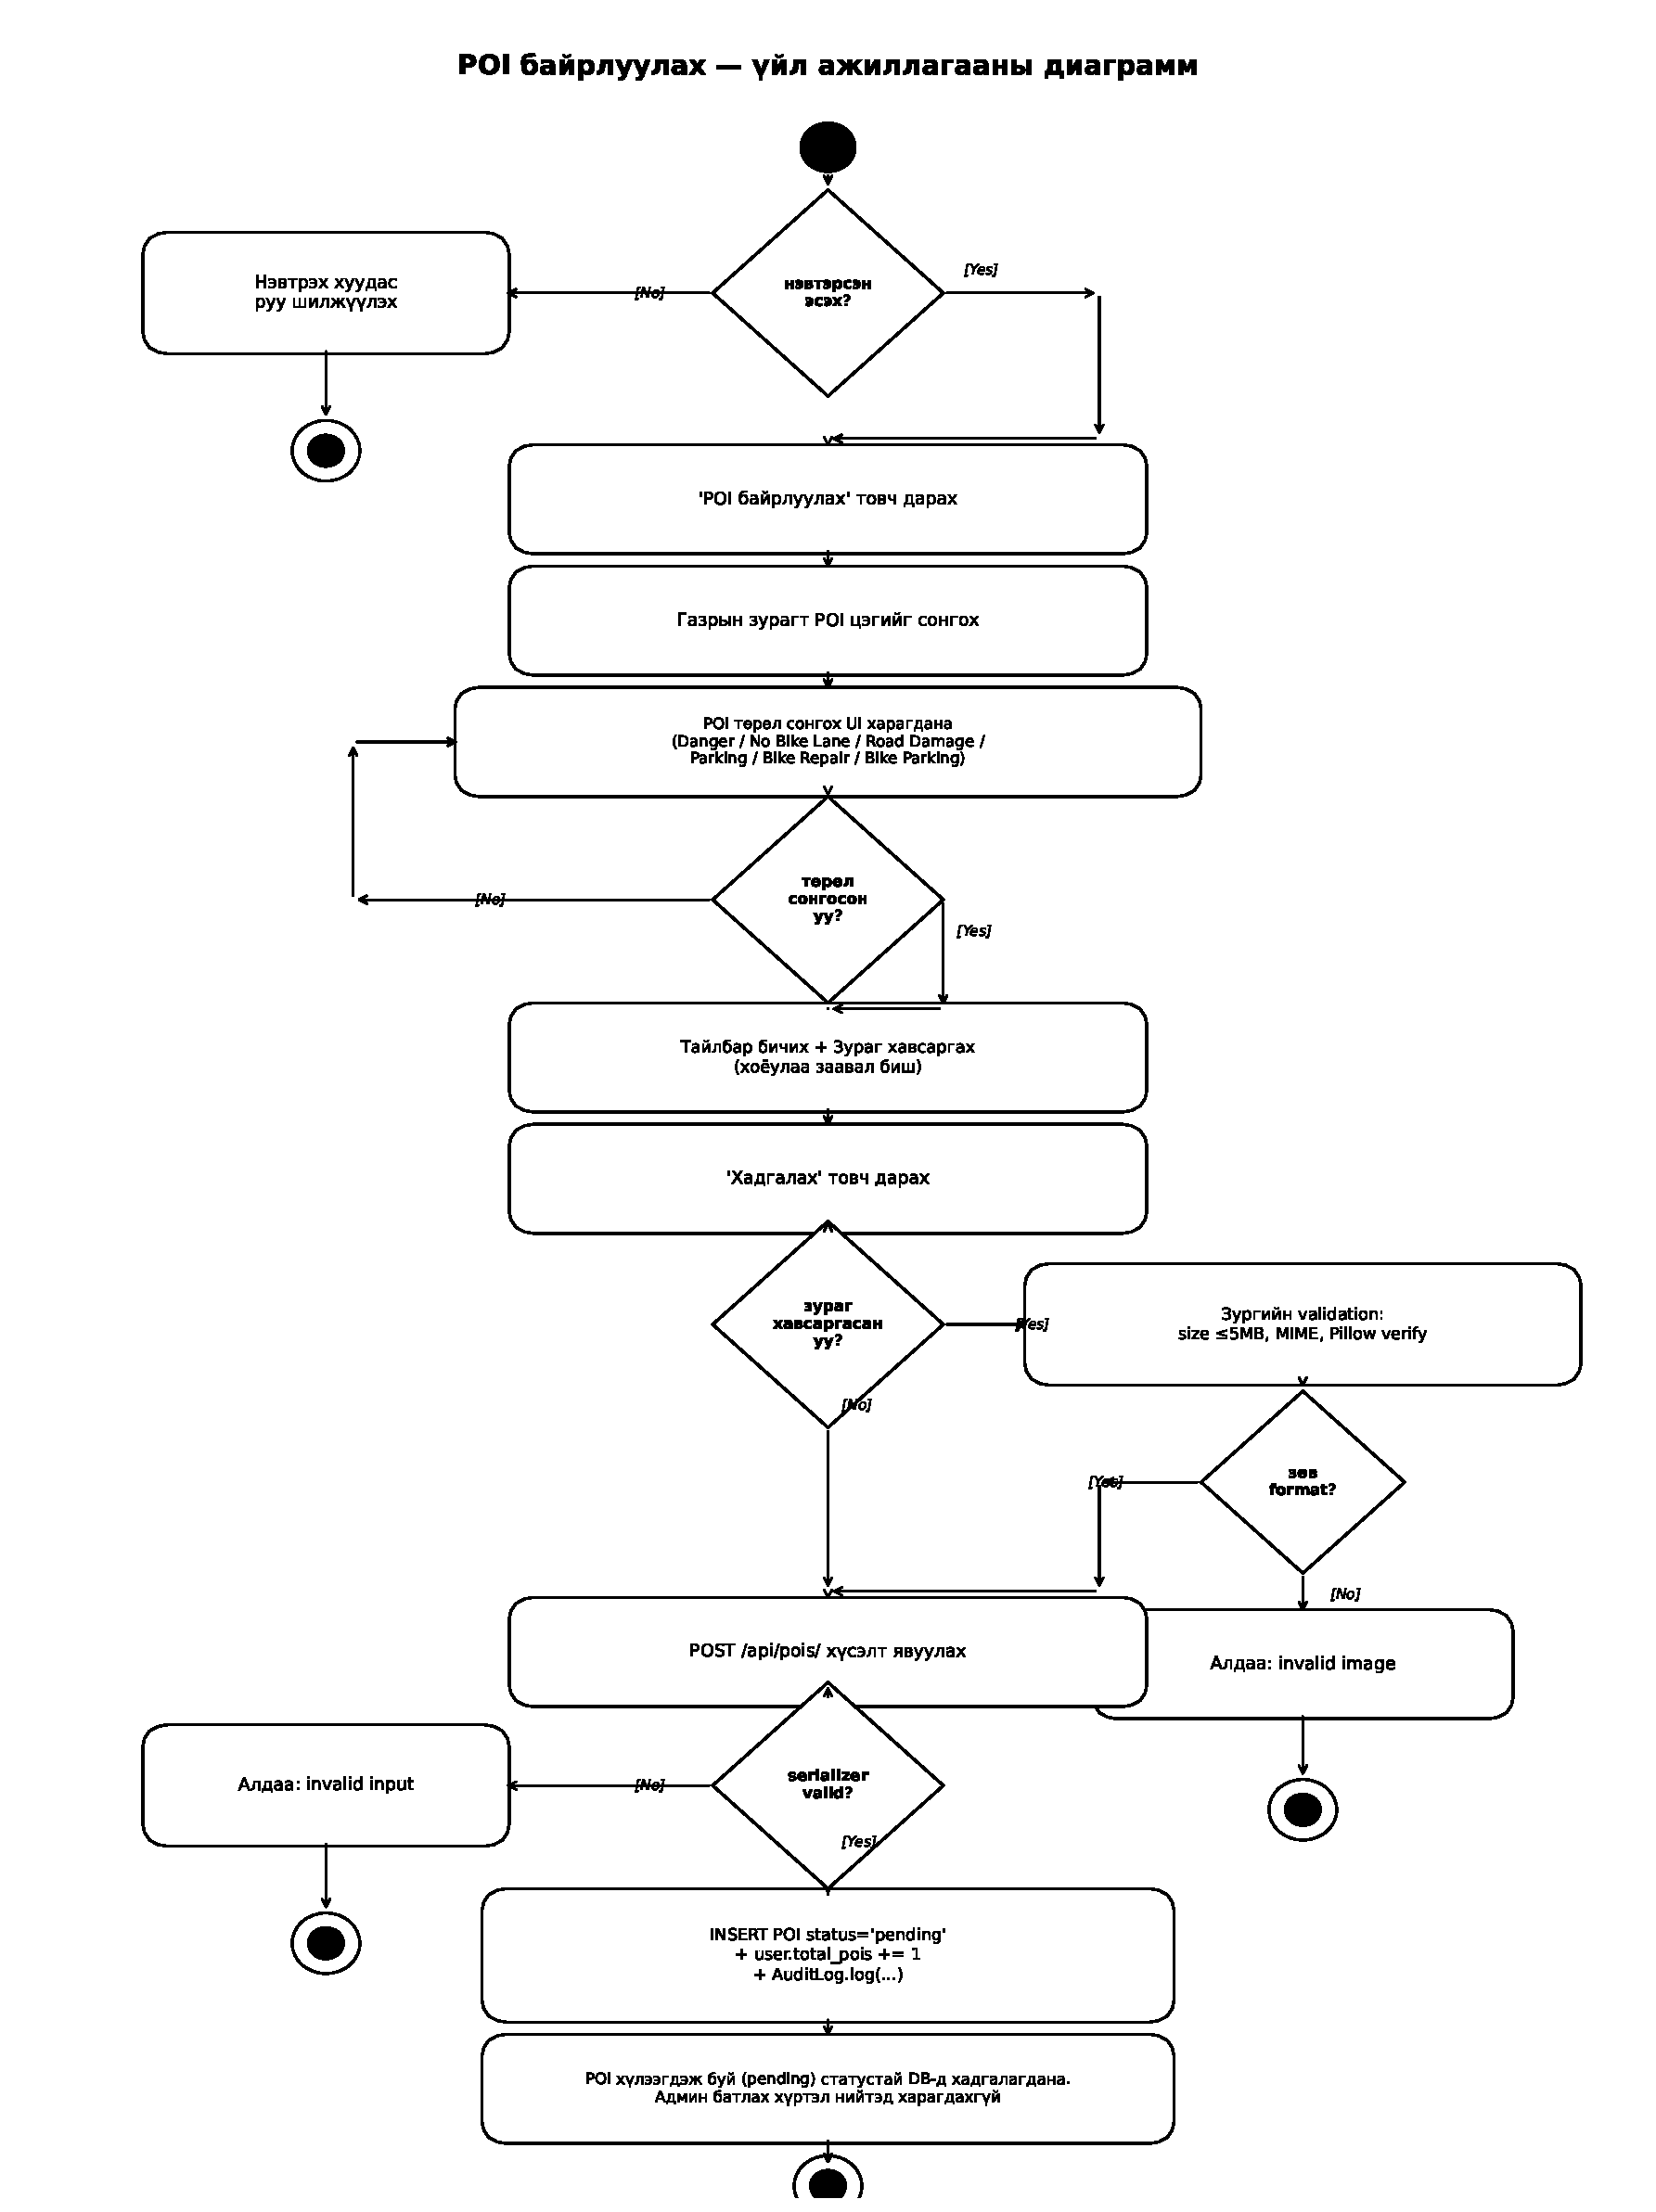
\includegraphics[scale=0.65]{Figures/chapter2/ua-poi.pdf} % auto-commented: missing file
    \caption{POI байрлуулах үйл ажиллагааны диаграмм}
    \label{fig:ua-poi}
\end{figure}
\par \noindent
Аюулгүй маршрут гаргах үйл ажиллагаа нь хэрэглэгч "Маршрут гаргах" товчийг дарснаар эхэлнэ. Эхлэл, төгсгөлийн цэгийг сонгож маршрутын төрлийг (Аюулгүй / Хурдан) сонгоно. Систем OSRM серверээс боломжит замуудыг авч crowd aggregation болон POI өгөгдөлд тулгуурлан өртгийг тооцоолон хамгийн оновчтой замыг газрын зурагт ногоон/шар/улаан өнгөөр харуулна. Дээрх процессыг Зураг \ref{fig:ua-route} -н аюулгүй маршрут гаргах үйл ажиллагааны диаграммаас харж болно.
\begin{figure}[H]
    \centering
    % 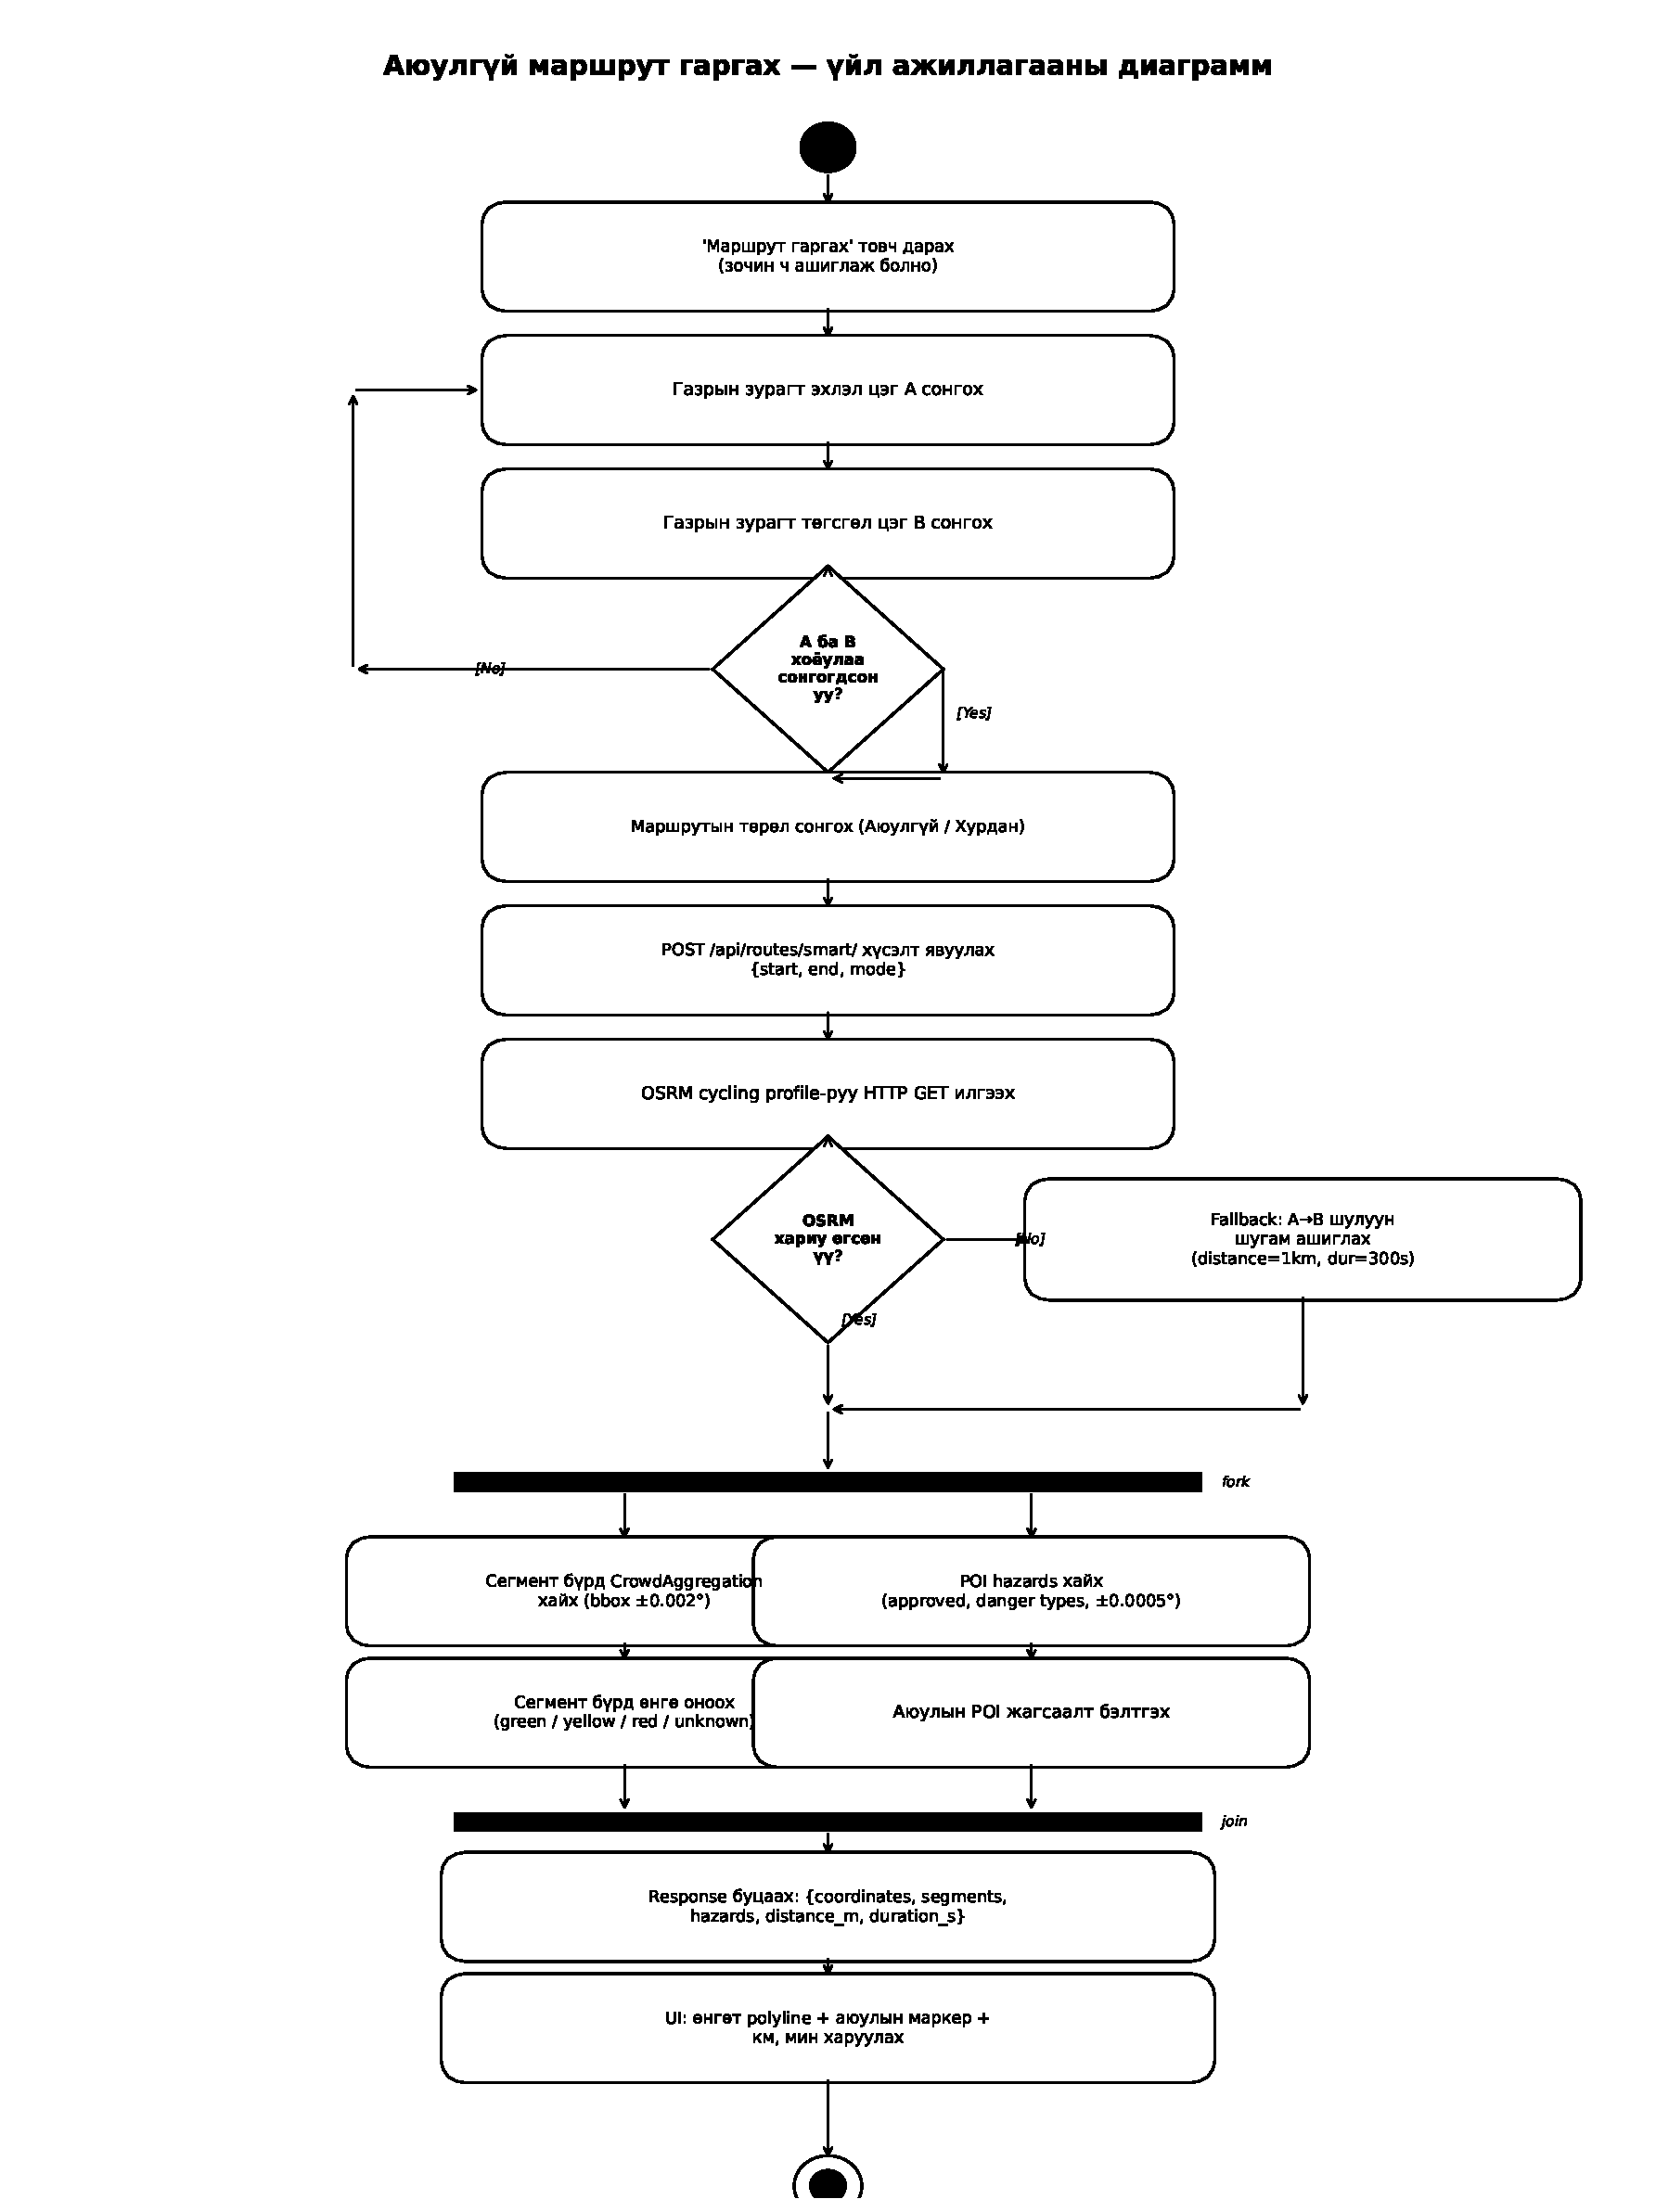
\includegraphics[scale=0.65]{Figures/chapter2/ua-route.pdf} % auto-commented: missing file
    \caption{Аюулгүй маршрут гаргах үйл ажиллагааны диаграмм}
    \label{fig:ua-route}
\end{figure}
\par \noindent

\section{Бүлгийн дүгнэлт}
\paragraph{} Энэ бүлэгт BikeMap UB системийн үйл ажиллагааг дэлгэрэнгүй тайлбарлаж, системийг ашиглах хэрэглэгчид болон шаардлагуудыг тодорхойлж, юзкейс, юзкейсийн тодорхойлолт болон шинжилгээний шатны класс, дараалал, үйл ажиллагааны диаграммуудыг гаргасан. Эхлээд системийг хэрэглэх зочин, бүртгэлтэй хэрэглэгч, админ гэсэн 3 төрлийн хэрэглэгчдийг тодорхойлоод тал бүрийн функцийн шаардлагыг тодорхойлж мөн системийн функцийн бус шаардлагыг (responsive UI, GPS гүйцэтгэл, JWT/RBAC аюулгүй байдал, маршрутын нарийвчлал гэх мэт) тодорхойлсон. Системд оролцогчдын функцийн шаардлага дээр үндэслэн 3 тоглогчтой юзкейс диаграммыг байгуулж, гол юзкейсүүдэд (Замын нөхцөл тэмдэглэх, POI байрлуулах, Аюулгүй маршрут гаргах) тодорхойлолт гаргасан. Юзкейсийг хэрэгжүүлж болох шинжилгээний шатны 6 классуудыг (Crowd Aggregation, Smart Route, Сегмент, POI, Хэрэглэгч, Бүртгэл) гаргаж тэдгээрийн холбоо хамаарлыг тодорхойлсон. Тодорхойлогдсон классууд болон юзкейсийн тодорхойлолтын дагуу дарааллын диаграмм болон үйл ажиллагааны диаграммуудыг гаргаж системийн үйл ажиллагаа, оролцогч талууд, процессын дарааллыг шинжилгээний түвшинд ойлгох боломжийг олгосон.
